\documentclass[11pt]{article}
\usepackage[margin=1in]{geometry}
\usepackage{amsmath,amssymb,amsthm}
\usepackage{booktabs}
\usepackage{enumitem}
\usepackage{xcolor}
\usepackage[colorlinks=true,linkcolor=blue!50!black,urlcolor=blue!50!black,citecolor=blue!50!black]{hyperref}
\usepackage{microtype}
\usepackage{tikz}
\usetikzlibrary{calc}
\usepackage{pdflscape}
\usepackage{graphicx}
% shared TikZ macros for the geometry figures (unit cells; source cell at the origin, target cell at the offset)
\newcommand{\cube}[3]{%
 \draw[gray!55,thin] (#1,#2,#3) -- ++(1,0,0) -- ++(0,1,0) -- ++(-1,0,0) -- cycle;
 \draw[gray!55,thin] (#1,#2,#3+1) -- ++(1,0,0) -- ++(0,1,0) -- ++(-1,0,0) -- cycle;
 \draw[gray!55,thin] (#1,#2,#3) -- ++(0,0,1) (#1+1,#2,#3) -- ++(0,0,1) (#1+1,#2+1,#3) -- ++(0,0,1) (#1,#2+1,#3) -- ++(0,0,1);}
\newcommand{\facex}[4]{\fill[#4,opacity=0.40] (#1,#2,#3) -- ++(0,1,0) -- ++(0,0,1) -- ++(0,-1,0) -- cycle; \draw[#4,thick] (#1,#2,#3) -- ++(0,1,0) -- ++(0,0,1) -- ++(0,-1,0) -- cycle;}
\newcommand{\facey}[4]{\fill[#4,opacity=0.40] (#2,#1,#3) -- ++(1,0,0) -- ++(0,0,1) -- ++(-1,0,0) -- cycle; \draw[#4,thick] (#2,#1,#3) -- ++(1,0,0) -- ++(0,0,1) -- ++(-1,0,0) -- cycle;}
\newcommand{\facez}[4]{\fill[#4,opacity=0.40] (#2,#3,#1) -- ++(1,0,0) -- ++(0,1,0) -- ++(-1,0,0) -- cycle; \draw[#4,thick] (#2,#3,#1) -- ++(1,0,0) -- ++(0,1,0) -- ++(-1,0,0) -- cycle;}
\newcommand{\axes}{\draw[->,gray] (-0.3,-0.3,0) -- ++(0.5,0,0) node[right,gray,font=\tiny]{$x$}; \draw[->,gray] (-0.3,-0.3,0) -- ++(0,0.5,0) node[above right,gray,font=\tiny]{$y$}; \draw[->,gray] (-0.3,-0.3,0) -- ++(0,0,0.5) node[above,gray,font=\tiny]{$z$};}
\tikzset{geo/.style={x={(0.95cm,-0.28cm)}, y={(0.62cm,0.42cm)}, z={(0cm,0.95cm)}, scale=1.0, every node/.style={font=\footnotesize}}}


\newtheorem{theorem}{Theorem}[section]
\newtheorem{proposition}[theorem]{Proposition}
\newtheorem{lemma}[theorem]{Lemma}
\newtheorem{corollary}[theorem]{Corollary}
\theoremstyle{remark}
\newtheorem{remark}[theorem]{Remark}

\newcommand{\dd}{\mathrm{d}}
\newcommand{\ii}{\mathrm{i}}
\newcommand{\asinh}{\operatorname{asinh}}
\newcommand{\atan}{\operatorname{atan}}
\newcommand{\Rr}{\mathbb{R}}
\newcommand{\code}[1]{\texttt{#1}}
\newcommand{\Gs}{G_{\mathrm{s}}}

\title{The Integrals of Gila:\\ What They Are, Which Are Analytic, and How to Finish the Rest}
\author{Claude (Anthropic, Claude Fable 5.1)\\[2pt]\small prepared for Paul Virally, GilaElectromagnetics}
\date{5 September 2026}

\begin{document}
\maketitle

\begin{abstract}
GilaElectromagnetics discretizes the electromagnetic volume integral equation on a
lattice of cuboid cells. Every entry of the discretized vacuum Green operator is a
sum of four-dimensional integrals of the scalar Helmholtz kernel over pairs of
rectangular cell faces. This document explains where those integrals come from, lists
exactly which of them Gila now evaluates in closed form and which it still evaluates
numerically, proves that a much larger class of them is elementary than the code
currently exploits, shows that the remaining ones are not elementary, works out exactly which special
functions they reduce to (incomplete Hankel functions for coplanar pairs, apparently a
genuinely two-variable function for perpendicular ones) and why the power series in
$k$ is nevertheless the right representation in Gila's regime, and collects the techniques, numerical measurements,
and pitfalls learned while deriving and hardening the closed forms during the
September 2026 work on the \code{paul-fp32} and \code{paul-metal} branches. It is
written to be self-contained so that the derivation of the remaining closed forms can
be taken up in a fresh session.
\end{abstract}

\tableofcontents

\section{How to read this document, and context for a fresh session}

\paragraph{The repository.} The relevant code lives in \code{src/vacuum/}:
\begin{itemize}[nosep]
\item \code{glaVacOprMemGen.jl} assembles the Green operator: the face-pair
bookkeeping (\code{facPar}, \code{srfSum!}, \code{srfScl}), the fixed
Gauss--Legendre rules for separated cells (\code{egoSrfFxd!}, \code{quadOrd},
\code{cntOrd}), the singular-cell corrections (\code{egoFunSng!}), and the memo of
weak integrals (\code{wekTrp}, \code{wekMem}).
\item \code{glaVacOprMemInt.jl} holds the scalar kernels (\code{sclEgo\_},
\code{sclEgoN\_}), the closed-form $1/r$ panel integrals (\code{rSrfSlf},
\code{rSrfEdgFlt}, \code{rSrfEdgCrn}), and the heads of the weakly singular
integrals (\code{wekS}, \code{wekE}, \code{wekV} and their \code{Dir} variants).
\item \code{glaVacOprMemIntSup.jl} is a Julia translation of DIRECTFN
\cite{directfn}, the fully numerical scheme for the singular remainders.
\end{itemize}
Tests for the closed forms are in \code{test/quadTest.jl} (testset ``Panel
Integrals''), and the convergence check of the weak integrals is
\code{test/vacuum/intConTest.jl}. The validation scripts of the studies summarized here are kept in \code{notes/gen/ref/}:
\code{mom.jl} is the high-precision evaluator of every panel-pair moment
(Section~\ref{sec:evaluator}), \code{mom7.jl} the general self-face moment formula with
its recurrence and cancellation-free form, \code{ref.jl} and \code{formsG.jl} the
$1/r$ closed forms, \code{slf.jl} and \code{dec.jl} the special-function reduction of
the self face, and \code{moments\_report.md} the analysis behind
Section~\ref{sec:momall}. The generator scripts for the figures, tables and the
appendix are in \code{notes/gen/}.

\paragraph{Conventions.} Lengths are measured in wavelengths. The frequency enters
through a single complex scalar $f$, the field \code{frqPhz} of the kernel options,
so that the wavenumber is $k = 2\pi f$. Gila's scalar kernel is
\begin{equation}
g(r) \;=\; \frac{e^{2\pi \ii f r}}{4\pi f^{2} r}
\;=\; \frac{e^{\ii k r}}{4\pi f^{2} r},
\qquad r = |\mathbf{x}-\mathbf{y}|,
\label{eq:kernel}
\end{equation}
and its regularized companion, used inside the singular integrals, is
$g_{\mathrm{N}}(r) = g(r) - 1/(4\pi f^2 r) = (e^{\ii k r}-1)/(4\pi f^2 r)$.
A cell has edge lengths $\mathbf{s} = (s_1, s_2, s_3)$, stored as exact
\code{Rational}s (the field \code{scl}). When a formula involves a single face I
write its edges as $l_a, l_b$ and a third length $l_c$ for the perpendicular
direction, matching the argument names of the \code{rSrf*} functions.

\paragraph{Frequency dependence.} Every integral of $1/r$ is proportional to $1/f^2$
and nothing else. This trivial fact turned out to matter (Section~\ref{sec:bug}).

\section{Where the integrals come from}
\label{sec:origin}

\subsection{From Maxwell to the volume integral equation}

In the frequency domain, a scatterer described by a susceptibility $\chi$ inside a
region $\Omega$ produces a total field $E$ satisfying
\begin{equation}
E = E^{\mathrm{inc}} + k^2 \int_{\Omega} \mathbf{G}(\mathbf{x}-\mathbf{y})\,
\chi(\mathbf{y})\, E(\mathbf{y})\,\dd\mathbf{y},
\end{equation}
where $\mathbf{G}$ is the dyadic Green function of free space. Gila solves this
equation for the polarization current $P = \chi E$, in the form
$(\mathbf{I} - \chi\,\mathbf{G}_0)\,\cdot = \cdot$ with $\mathbf{G}_0$ the
discretized vacuum Green operator, which is why the memory notes refer to the
``$(I - X G_0)$ solve''. The dyadic Green function is
\begin{equation}
\mathbf{G}(\mathbf{r}) \;=\; \Bigl(\mathbf{I} + \frac{\nabla\nabla}{k^2}\Bigr)\Gs(r),
\qquad
\Gs(r) = \frac{e^{\ii k r}}{4\pi r},
\qquad (\nabla^2 + k^2)\,\Gs = -\delta(\mathbf{r}).
\label{eq:dyadic}
\end{equation}
Using the Helmholtz equation to replace $\Gs$ in the identity term,
$\Gs\,\mathbf{I} = -(\mathbf{I}\nabla^2 \Gs + \mathbf{I}\delta)/k^2$, one gets the
form Gila actually uses,
\begin{equation}
\mathbf{G}(\mathbf{r}) \;=\; \frac{1}{k^2}\bigl(\nabla\nabla - \mathbf{I}\,\nabla^2\bigr)\Gs(r)
\;-\; \frac{\mathbf{I}}{k^2}\,\delta(\mathbf{r}).
\label{eq:curlcurl}
\end{equation}
Component-wise, with $\partial_a = \partial/\partial x_a$,
\begin{equation}
G_{ab} = \frac{1}{k^2}\Bigl(\partial_a\partial_b - \delta_{ab}\sum_c \partial_c\partial_c\Bigr)\Gs - \frac{\delta_{ab}}{k^2}\,\delta,
\qquad\text{e.g.}\quad
G_{xx} = -\frac{\partial_y\partial_y + \partial_z\partial_z}{k^2}\,\Gs - \frac{\delta}{k^2},
\quad
G_{xy} = \frac{\partial_x\partial_y}{k^2}\,\Gs .
\end{equation}

\subsection{Cell averaging and the divergence theorem, twice}

Gila uses piecewise-constant basis functions on cuboid cells with Galerkin testing,
so the entry of $\mathbf{G}_0$ coupling a source cell $V_s$ to a target cell $V_t$
is the double volume average
\begin{equation}
(\mathbf{G}_0)_{ab}(t,s) \;=\; \frac{1}{V_t}\int_{V_t}\!\int_{V_s}
G_{ab}(\mathbf{x}-\mathbf{y})\,\dd\mathbf{y}\,\dd\mathbf{x}.
\label{eq:cellavg}
\end{equation}
The derivatives in \eqref{eq:curlcurl} are what make this tractable. Because $\Gs$
depends on $\mathbf{x}-\mathbf{y}$, a derivative with respect to $y_b$ is minus the
derivative with respect to $x_b$, so
$\partial_a\partial_b\Gs(\mathbf{x}-\mathbf{y}) = -\partial^{x}_a\partial^{y}_b\Gs$.
Each derivative can now be moved onto its own integration domain by the divergence
theorem, turning a volume integral into a surface integral over the cell boundary:
\begin{equation}
\int_{V_t}\!\int_{V_s}\partial_a\partial_b\Gs\,\dd\mathbf{y}\,\dd\mathbf{x}
\;=\; -\oint_{\partial V_t}\!\oint_{\partial V_s} n_a(\mathbf{x})\,n'_b(\mathbf{y})\,
\Gs(|\mathbf{x}-\mathbf{y}|)\,\dd S'\,\dd S,
\label{eq:divdiv}
\end{equation}
where $\mathbf{n}$ and $\mathbf{n}'$ are the outward normals of the target and source
cells. Every second derivative of the singular kernel has become a
\emph{surface--surface integral of the scalar kernel itself}, which is only weakly
singular ($1/r$ on a four-dimensional domain, integrable). This is the whole reason
Gila computes surface integrals: the volume--volume integral of the strongly singular
dyadic has been traded for surface--surface integrals of $\Gs$.

For a cuboid cell the boundary consists of six rectangles, each with a constant
normal $\pm\mathbf{e}_c$. The double surface integral therefore splits into $6\times 6
= 36$ \emph{face-pair integrals}
\begin{equation}
I_{FF'} \;=\; \int_{F}\!\int_{F'} \Gs(|\mathbf{x}-\mathbf{y}|)\,\dd S'\,\dd S,
\qquad F\subset\partial V_t,\; F'\subset\partial V_s,
\label{eq:facepair}
\end{equation}
and the tensor components are signed sums of them. Writing $\sigma_F = \pm 1$ for the
sign of the normal of face $F$ and $c(F)$ for its axis,
\begin{align}
(\mathbf{G}_0)_{aa} &= \frac{1}{k^2 V_t}\sum_{\substack{F,F'\\ c(F)=c(F')\neq a}}
\sigma_F\,\sigma_{F'}\, I_{FF'} \;-\; \frac{\delta_{ts}}{k^2}, \\
(\mathbf{G}_0)_{ab} &= -\frac{1}{k^2 V_t}\sum_{\substack{F,F'\\ c(F)=a,\; c(F')=b}}
\sigma_F\,\sigma_{F'}\, I_{FF'}, \qquad a\neq b .
\end{align}
Appendix~\ref{app:36} writes all 36 integrals out with explicit limits, and the nine
signed sums. This is exactly what \code{srfSum!} does. Its face ordering is
\code{yzL yzU xzL xzU xyL xyU} (faces 1--6, L and U for the lower and upper face on
each axis) and the face-pair index is $36$-long with $\mathrm{fp} = 6(F-1)+F'$. For
example the $xx$ entry is
\code{srfMat[15]-[16]-[21]+[22]+[29]-[30]-[35]+[36]}: pairs 15, 16, 21, 22 are the
four combinations of the two $y$-faces of the target with the two $y$-faces of the
source, with signs $\sigma_F\sigma_{F'}$, and 29--36 likewise for the $z$-faces. The
$xy$ entry \code{-[3]+[4]+[9]-[10]} pairs the $x$-faces of the target with the
$y$-faces of the source, with the overall minus sign of \eqref{eq:divdiv}.

The constant prefactors are absorbed into Gila's kernel \eqref{eq:kernel} and its
normalizations. The face-pair integrand is evaluated over the unit hypercube
$[0,1]^4$ and rescaled by \code{srfScl}, which is (source face area)/(target
edge normal to the target face), i.e.\ the areas of both faces divided by the target
volume. The weak integrals returned by \code{wekS}, \code{wekE}, \code{wekV} are raw
integrals $\int_F\int_{F'} g$ over the full rectangles and are divided by the cell
volume in \code{wekTrp}. The identity term $-\delta_{ab}\,\delta_{ts}/k^2$ appears as
the three lines \code{egoToe[i,i,1,1,1] -= 1/frqPhz\textasciicircum 2} in
\code{genEgoCrcSlf!}, which fixes the relation between Gila's overall constant and the
physical one: Gila's operator equals $4\pi^2$ times \eqref{eq:cellavg} in units where
the wavelength is one.

\subsection{Why so few distinct integrals are needed}

On a regular grid the interaction depends only on the relative offset of the two
cells, so $\mathbf{G}_0$ is block Toeplitz and is applied with FFTs. Generation
therefore needs one $3\times 3$ tensor per relative offset, and each tensor needs 36
face-pair integrals. Moreover the face pairs of offset cells are all axis-aligned
rectangle pairs of a small number of \emph{types}, determined by whether the
rectangles are coplanar or perpendicular and by how they touch. This is what makes
closed forms worth having: a handful of formulas, evaluated once per cell shape,
cover every contact interaction in the volume.

\subsection{The anti-Hermitian part as a physical check}
\label{sec:asym}

For real $f$ the panel integrals of $1/r$ are real, and the anti-Hermitian part
$\operatorname{asym}\mathbf{G}_0 = (\mathbf{G}_0 - \mathbf{G}_0^\dagger)/2\ii$ of a
Toeplitz operator with an even kernel is the Toeplitz operator of the imaginary part
of the kernel. Passivity requires $\operatorname{asym}\mathbf{G}_0 \succeq 0$. This
gives a useful end-to-end test of the whole assembly, because it is sensitive only to
the imaginary parts and to the frequency prefactors, and it was how the severity of
the bug of Section~\ref{sec:bug} became visible: on a $6^3$ cell block at
$f = 1 + 0.1\ii$ the buggy operator had $\lambda_{\min}(\operatorname{asym}\mathbf{G}_0)
= -0.485$ against $\lambda_{\max} = 0.28$; after the fix all eigenvalues are positive.
At real frequency, both before and after, $\lambda_{\min}$ sits at the rounding floor
($-5\times 10^{-15}$ against $\lambda_{\max} = 0.077$), because the $1/r$ terms do not
enter it at all.

\section{A taxonomy of the integrals Gila computes}
\label{sec:taxonomy}

All integrals are of the form \eqref{eq:facepair} with the kernel $g$ of
\eqref{eq:kernel}. They differ only in the relative position of the two rectangles,
and Gila treats them by three methods.

\subsection{Contact integrals: rectangles that touch}
\label{sec:contact}

When the two cells coincide or share a face, an edge, or a vertex, some of their 36
face pairs touch, and the kernel's $1/r$ is on the integration domain. For a regular
grid the touching pairs fall into five geometries, illustrated with the source cell
$[0,l_a]\times[0,l_b]\times[0,l_c]$:
\begin{description}[nosep,leftmargin=1.5em]
\item[Self (coincident faces).] The same face with itself (self cell), or the upper
$x$-face of the source with the lower $x$-face of a target displaced by one cell in
$x$: these are the same rectangle. Called \code{wS} in the code; closed form
\code{rSrfSlf}$(l_a,l_b)$ for the $1/r$ part.
\item[Flat edge (coplanar, sharing an edge).] The lower $y$-faces of two cells
adjacent in $x$: coplanar rectangles $[0,l_a]\times[0,l_c]$ and
$[l_a,2l_a]\times[0,l_c]$ sharing the edge of length $l_c$. Called \code{wE} entries
1--6 (\code{xxY, xxZ, yyX, yyZ, zzX, zzY}); closed form
\code{rSrfEdgFlt}$(l_{\text{shared}}, l_{\text{width}})$, whose second argument is
``doubled'': the two panels together span twice its length.
\item[Cornered edge (perpendicular, sharing an edge).] Two faces of the same cell
that meet at an edge, or the upper $y$-face of the source with the lower $x$-face of a
target displaced by $(1,1,0)$ cells. Called \code{wE} entries 7--9 (\code{xy, xz,
yz}); closed form \code{rSrfEdgCrn}$(l_{\text{shared}}, l_b, l_c)$. \code{wekE}
computes each of these twice in the two orientations (\code{xyA}, \code{xyB}) and
averages, which is why the numerical symmetry of the closed form under $l_b
\leftrightarrow l_c$ mattered.
\item[Coplanar vertex (coplanar, sharing a corner).] The lower $z$-faces of two
cells adjacent along the $(1,1,0)$ diagonal. Called \code{wV} entries 1--3. No closed
form; DIRECTFN on the full kernel.
\item[Perpendicular vertex (perpendicular planes, sharing a corner).] The upper
$z$-face of the source with the lower $x$-face of a target displaced by $(1,1,1)$
cells. Called \code{wV} entries 4--6, also averaged over two orientations. No closed
form.
\end{description}

Figure~\ref{fig:contact} draws each geometry with both cells, and Table~\ref{tab:class}
classifies all 36 face pairs for the four distinct kinds of touching cell pairs (face
neighbour, edge neighbour, vertex neighbour, and the cell itself; the other 22
neighbours are these up to reflection). The letter codes are: S coincident, Ef flat
edge, Ec cornered edge, Vc coplanar vertex, Vp perpendicular vertex, and for the
non-touching pairs of Section~\ref{sec:shell} P1/P2 parallel one or two cell lengths
apart, a suffix s for a lateral shift, and Xg perpendicular planes that do not meet.
The tables were generated mechanically from the face definitions and agree entry by
entry with the correction masks hard-coded in \code{egoFunSng!} (mask $1$ = one of
S, Ef, Ec, Vc, Vp; mask $0$ = one of P1, P2, P1s, P2s, Xg).

\begin{figure}[htbp]
\begin{center}\footnotesize
\begin{tabular}{@{}ccc@{}}
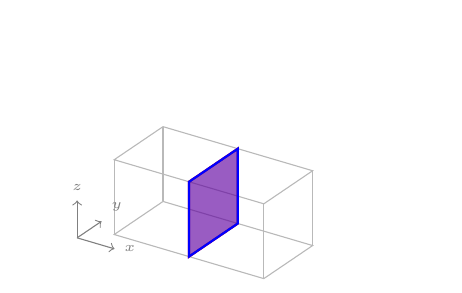
\begin{tikzpicture}[geo]\useasboundingbox (-0.7,-0.7,-0.3) rectangle (2.7,2.4,2.5); \cube{0}{0}{0}\cube{1}{0}{0} \facex{1}{0}{0}{red} \facex{1}{0}{0}{blue} \axes\end{tikzpicture} & 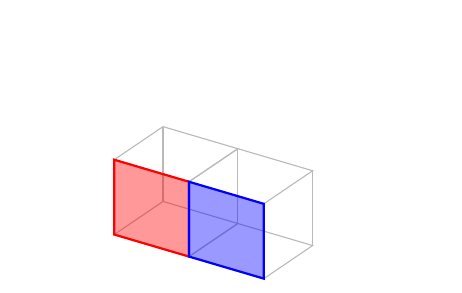
\begin{tikzpicture}[geo]\useasboundingbox (-0.7,-0.7,-0.3) rectangle (2.7,2.4,2.5); \cube{0}{0}{0}\cube{1}{0}{0} \facey{0}{0}{0}{red} \facey{0}{1}{0}{blue}\end{tikzpicture} & 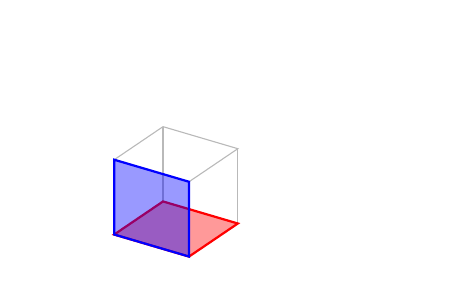
\begin{tikzpicture}[geo]\useasboundingbox (-0.7,-0.7,-0.3) rectangle (2.7,2.4,2.5); \cube{0}{0}{0} \facez{0}{0}{0}{red} \facey{0}{0}{0}{blue}\end{tikzpicture} \\[2pt]
\parbox{0.31\textwidth}{\centering\textbf{S}: coincident\\ {\scriptsize $\Delta=(1,0,0)$: yzL of target, yzU of source}} & \parbox{0.31\textwidth}{\centering\textbf{Ef}: flat edge, coplanar\\ {\scriptsize $\Delta=(1,0,0)$: xzL of target, xzL of source}} & \parbox{0.31\textwidth}{\centering\textbf{Ec}: cornered edge, perpendicular\\ {\scriptsize $\Delta=0$: xzL and xyL of the same cell}} \\[10pt]
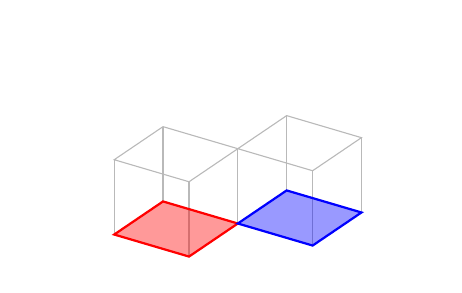
\begin{tikzpicture}[geo]\useasboundingbox (-0.7,-0.7,-0.3) rectangle (2.7,2.4,2.5); \cube{0}{0}{0}\cube{1}{1}{0} \facez{0}{0}{0}{red} \facez{0}{1}{1}{blue}\end{tikzpicture} & 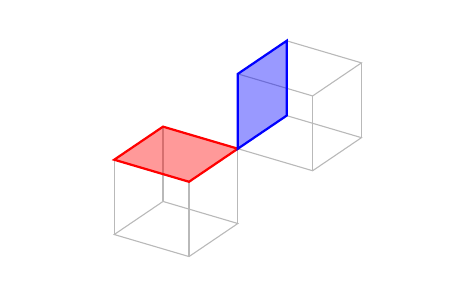
\begin{tikzpicture}[geo]\useasboundingbox (-0.7,-0.7,-0.3) rectangle (2.7,2.4,2.5); \cube{0}{0}{0}\cube{1}{1}{1} \facez{1}{0}{0}{red} \facex{1}{1}{1}{blue}\end{tikzpicture} & 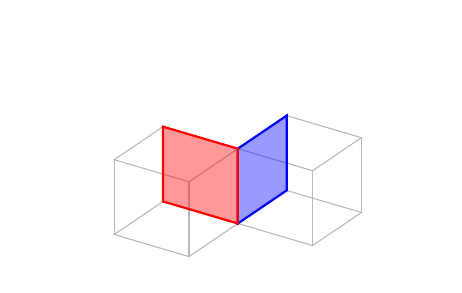
\begin{tikzpicture}[geo]\useasboundingbox (-0.7,-0.7,-0.3) rectangle (2.7,2.4,2.5); \cube{0}{0}{0}\cube{1}{1}{0} \facex{1}{1}{0}{blue} \facey{1}{0}{0}{red}\end{tikzpicture} \\[2pt]
\parbox{0.31\textwidth}{\centering\textbf{Vc}: coplanar vertex\\ {\scriptsize $\Delta=(1,1,0)$: xyL of target, xyL of source}} & \parbox{0.31\textwidth}{\centering\textbf{Vp}: perpendicular vertex\\ {\scriptsize $\Delta=(1,1,1)$: yzL of target, xyU of source}} & \parbox{0.31\textwidth}{\centering\textbf{Ec}: cornered edge across cells\\ {\scriptsize $\Delta=(1,1,0)$: yzL of target, xzU of source}} \\[10pt]
\end{tabular}\end{center}

\caption{The five contact geometries. Red: source face $F'$ (source cell at the
origin); blue: target face $F$ (target cell displaced by $\Delta$ cells). Where the two
faces coincide (S) the colours overlap. The cornered edge occurs both within one cell
and across diagonal neighbours.}
\label{fig:contact}
\end{figure}

\begin{table}[htbp]
\begin{center}\footnotesize\setlength{\tabcolsep}{3pt}
\begin{tabular}{@{}l|cccccc@{}}
\multicolumn{7}{@{}l}{$\Delta = (0,0,0)$}\\
$F\backslash F'$ & yzL & yzU & xzL & xzU & xyL & xyU\\ \hline
yzL & S & P1 & Ec & Ec & Ec & Ec\\
yzU & P1 & S & Ec & Ec & Ec & Ec\\
xzL & Ec & Ec & S & P1 & Ec & Ec\\
xzU & Ec & Ec & P1 & S & Ec & Ec\\
xyL & Ec & Ec & Ec & Ec & S & P1\\
xyU & Ec & Ec & Ec & Ec & P1 & S\\
\end{tabular}\hspace{6pt}
\begin{tabular}{@{}l|cccccc@{}}
\multicolumn{7}{@{}l}{$\Delta = (1,0,0)$}\\
$F\backslash F'$ & yzL & yzU & xzL & xzU & xyL & xyU\\ \hline
yzL & P1 & S & Ec & Ec & Ec & Ec\\
yzU & P2 & P1 & Xg & Xg & Xg & Xg\\
xzL & Xg & Ec & Ef & P1s & Vp & Vp\\
xzU & Xg & Ec & P1s & Ef & Vp & Vp\\
xyL & Xg & Ec & Vp & Vp & Ef & P1s\\
xyU & Xg & Ec & Vp & Vp & P1s & Ef\\
\end{tabular}\hspace{6pt}
\\[8pt]
\begin{tabular}{@{}l|cccccc@{}}
\multicolumn{7}{@{}l}{$\Delta = (1,1,0)$}\\
$F\backslash F'$ & yzL & yzU & xzL & xzU & xyL & xyU\\ \hline
yzL & P1s & Ef & Xg & Ec & Vp & Vp\\
yzU & P2s & P1s & Xg & Xg & Xg & Xg\\
xzL & Xg & Ec & P1s & Ef & Vp & Vp\\
xzU & Xg & Xg & P2s & P1s & Xg & Xg\\
xyL & Xg & Vp & Xg & Vp & Vc & P1s\\
xyU & Xg & Vp & Xg & Vp & P1s & Vc\\
\end{tabular}\hspace{6pt}
\begin{tabular}{@{}l|cccccc@{}}
\multicolumn{7}{@{}l}{$\Delta = (1,1,1)$}\\
$F\backslash F'$ & yzL & yzU & xzL & xzU & xyL & xyU\\ \hline
yzL & P1s & Vc & Xg & Vp & Xg & Vp\\
yzU & P2s & P1s & Xg & Xg & Xg & Xg\\
xzL & Xg & Vp & P1s & Vc & Xg & Vp\\
xzU & Xg & Xg & P2s & P1s & Xg & Xg\\
xyL & Xg & Vp & Xg & Vp & P1s & Vc\\
xyU & Xg & Xg & Xg & Xg & P2s & P1s\\
\end{tabular}\hspace{6pt}
\end{center}
\caption{Geometry of every face pair $(F, F')$, target face $F$ in rows and source
face $F'$ in columns, for the source cell itself and its three kinds of touching
neighbour. Codes as in the text.}
\label{tab:class}
\end{table}

The numerical method for the first three is a \emph{singularity subtraction}:
\begin{equation}
\int\!\!\int g \;=\; \underbrace{\frac{1}{4\pi f^2}\int\!\!\int \frac{1}{r}}_{\text{closed form}}
\;+\; \underbrace{\int\!\!\int \frac{e^{\ii k r}-1}{4\pi f^2 r}}_{\text{DIRECTFN, order \code{intOrd}}} .
\label{eq:split}
\end{equation}
The regularized kernel $g_{\mathrm{N}}$ is bounded (it tends to $\ii k/(4\pi f^2) =
\ii/(2 f)$ as $r\to 0$; the code evaluates it as $\ii\,\mathrm{cispi}(fr)\,\mathrm{sinc}(fr)/(2f)$
to avoid cancellation, see Section~\ref{sec:kernels}). DIRECTFN then integrates it by
splitting each rectangle into two triangles and applying a chain of variable
transformations that map the four-dimensional triangle-pair integral onto a smooth
integrand over a box, which is integrated by tensor Gauss--Legendre rules with
\code{intOrd} points per dimension. The default is now $\code{intOrd} = 48$, so a
self-face costs of order $48^4 \approx 5\times 10^6$ kernel evaluations. The vertex
integrals use DIRECTFN on the \emph{unregularized} kernel (the flag \code{sngMod =
false} in \code{wekVInt} selects \code{kerEV}, the full $g$), because the vertex
singularity is mild enough for the transformations alone.

\subsection{Touching-shell integrals: rectangles of touching cells that do not touch}
\label{sec:shell}

For a pair of touching cells most of the 36 face pairs do \emph{not} touch: they are
at least one cell length apart. Two faces of touching cells with the same normal axis
either lie in the same plane, in which case they are one of the contact geometries
above (coplanar faces of touching cells always meet, so a coplanar pair with a gap
never occurs on the lattice), or lie in parallel planes one or two cell lengths apart,
possibly shifted laterally by a cell length when the cells are diagonal neighbours.
Faces with different normal axes either share an edge or a vertex (contact) or sit in
perpendicular planes a cell length apart without meeting. These integrals are regular
but nearly singular, and Gila integrates them with a fixed Gauss--Legendre tensor rule
of order $\code{cntOrd} = 9$ (\code{pairListUn} in \code{egoFunSng!}; the mask tables
there mark them with a $0$). Figure~\ref{fig:shell} draws the five cases; their
counts per neighbour type can be read off Table~\ref{tab:class}: 6 of 36 for the cell
itself (all P1), 15 for a face neighbour, 22 for an edge neighbour, 27 for a vertex
neighbour.

\begin{figure}[htbp]
\begin{center}\footnotesize
\begin{tabular}{@{}ccc@{}}
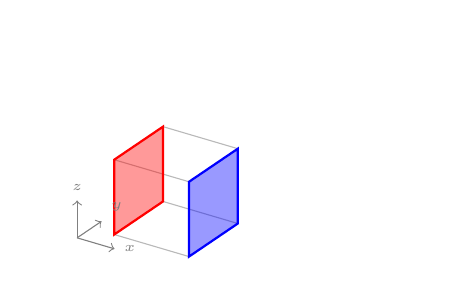
\begin{tikzpicture}[geo]\useasboundingbox (-0.7,-0.7,-0.3) rectangle (2.7,2.4,2.5); \cube{0}{0}{0} \facex{0}{0}{0}{red} \facex{1}{0}{0}{blue} \axes\end{tikzpicture} & 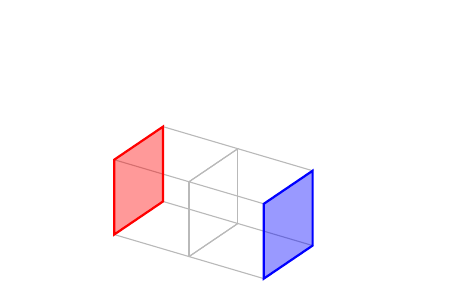
\begin{tikzpicture}[geo]\useasboundingbox (-0.7,-0.7,-0.3) rectangle (2.7,2.4,2.5); \cube{0}{0}{0}\cube{1}{0}{0} \facex{0}{0}{0}{red} \facex{2}{0}{0}{blue}\end{tikzpicture} & 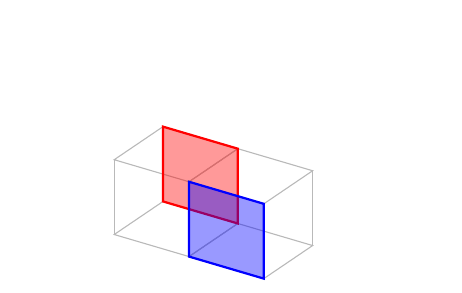
\begin{tikzpicture}[geo]\useasboundingbox (-0.7,-0.7,-0.3) rectangle (2.7,2.4,2.5); \cube{0}{0}{0}\cube{1}{0}{0} \facey{1}{0}{0}{red} \facey{0}{1}{0}{blue}\end{tikzpicture} \\[2pt]
\parbox{0.31\textwidth}{\centering\textbf{P1}: parallel, one cell apart\\ {\scriptsize $\Delta=0$: yzU of target, yzL of source}} & \parbox{0.31\textwidth}{\centering\textbf{P2}: parallel, two cells apart\\ {\scriptsize $\Delta=(1,0,0)$: yzU of target, yzL of source}} & \parbox{0.31\textwidth}{\centering\textbf{P1s}: parallel, one apart, shifted\\ {\scriptsize $\Delta=(1,0,0)$: xzL of target, xzU of source}} \\[10pt]
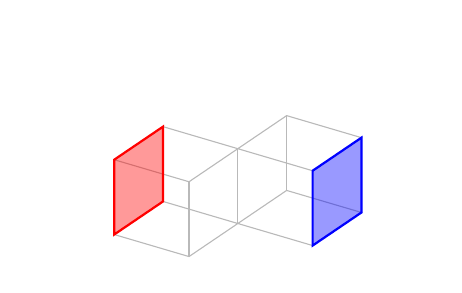
\begin{tikzpicture}[geo]\useasboundingbox (-0.7,-0.7,-0.3) rectangle (2.7,2.4,2.5); \cube{0}{0}{0}\cube{1}{1}{0} \facex{0}{0}{0}{red} \facex{2}{1}{0}{blue}\end{tikzpicture} & 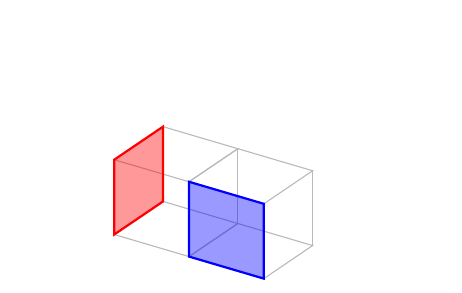
\begin{tikzpicture}[geo]\useasboundingbox (-0.7,-0.7,-0.3) rectangle (2.7,2.4,2.5); \cube{0}{0}{0}\cube{1}{0}{0} \facex{0}{0}{0}{red} \facey{0}{1}{0}{blue}\end{tikzpicture} \\[2pt]
\parbox{0.31\textwidth}{\centering\textbf{P2s}: parallel, two apart, shifted\\ {\scriptsize $\Delta=(1,1,0)$: yzU of target, yzL of source}} & \parbox{0.31\textwidth}{\centering\textbf{Xg}: perpendicular, not meeting\\ {\scriptsize $\Delta=(1,0,0)$: xzL of target, yzL of source}} \\[10pt]
\end{tabular}\end{center}

\caption{The five non-touching face-pair geometries that occur between touching
cells. Same colour convention as Figure~\ref{fig:contact}.}
\label{fig:shell}
\end{figure}

\subsection{Separated integrals: cells two or more apart}

For cells whose max-norm separation is at least two cells, every face pair is
separated by at least one cell length, and the integrand is smooth. Gila uses a fixed
tensor Gauss--Legendre rule whose order comes from the measured schedule in
\code{quadOrd}: 9 points per dimension at 2 cells, 7 at 3--4, 6 at 5--6, 5 at 7--16,
4 beyond, with a floor of 5 for cells above $\lambda/8$ and 6 above $\lambda/4$. The
schedule targets $10^{-10}$ relative error on the assembled tensor with one order of
margin. It was measured, not derived, and is described in the comment above
\code{quadOrd}. The measurement also showed why assembled accuracy is the right
target: \code{srfSum!} subtracts face pairs of nearly equal size, amplifying
face-pair error by a factor between 10 and 1000, so a face pair must be good to
$10^{-12}$--$10^{-13}$ for the tensor to be good to $10^{-10}$.

Cross-scale volume pairs whose cells are not aligned to a common lattice fall
through to adaptive cubature (\code{egoSrfAdp!}, HCubature); these are rare and not
discussed further.

\subsection{Summary table}

\begin{center}
\footnotesize
\begin{tabular}{@{}lllll@{}}
\toprule
Geometry & Kernel part & Method today & Analytic? & Analytic possible? \\
\midrule
Self face & $1/r$ & closed form \code{rSrfSlf} & yes & --- \\
Self face & $(e^{\ii kr}-1)/r$ & DIRECTFN, order 48 & no & yes, series (Sec.~\ref{sec:theorem}, \ref{sec:momall}) \\
Flat edge & $1/r$ & closed form \code{rSrfEdgFlt} & yes & --- \\
Flat edge & $(e^{\ii kr}-1)/r$ & DIRECTFN & no & yes, series \\
Cornered edge & $1/r$ & closed form \code{rSrfEdgCrn} & yes & --- \\
Cornered edge & $(e^{\ii kr}-1)/r$ & DIRECTFN & no & yes, series \\
Coplanar vertex & $e^{\ii kr}/r$ & DIRECTFN, full kernel & no & yes: $1/r$ closed form + series \\
Perpendicular vertex & $e^{\ii kr}/r$ & DIRECTFN, full kernel & no & yes: $1/r$ closed form + series \\
Parallel offset $1\times$, $2\times$ & $e^{\ii kr}/r$ & GL order 9 & no & yes, series (measured) \\
Parallel, laterally shifted & $e^{\ii kr}/r$ & GL order 9 & no & yes, series (expected) \\
Perpendicular, not meeting & $e^{\ii kr}/r$ & GL order 9 & no & yes, series (expected) \\
Separated $\ge 2$ cells & $e^{\ii kr}/r$ & GL order 4--9 & no & not usefully (Sec.~\ref{sec:far}) \\
\bottomrule
\end{tabular}
\end{center}

\section{What has been done analytically}
\label{sec:done}

Only the $1/r$ parts of the self, flat-edge and cornered-edge integrals are closed
form. These three formulas existed in Gila from its first commit as
Mathematica-generated expressions of 20--30 terms in logarithms, square roots, and
inverse trigonometric functions. In September 2026 they were replaced by short
equivalent forms derived by hand, for two reasons: one of them was wrong for complex
frequency, and all three lost most of their digits for slender panels. This section
records the derivations, since they are the templates for what remains.

\subsection{The difference-variable reduction}
\label{sec:diffvar}

The central trick for coplanar rectangles is to integrate over the \emph{difference}
of the two points rather than the points themselves. Let the target panel be
$A = [0,p]$ in one coordinate and the source panel $B = [c, c+p']$. The kernel depends
only on $u = x' - x$. For fixed $u$, the measure of pairs $(x, x')\in A\times B$ with
$x'-x = u$ is the convolution of the two indicator functions, a trapezoid in $u$: for
two equal intervals with the same origin it is the triangle $p - |u|$ on $[-p,p]$; for
adjacent intervals $[0,p]$ and $[p,2p]$ it is the triangle $p - |u - p|$ centred at
$u = p$; for an interval against a degenerate one (a point, when the other rectangle
lies in a perpendicular plane) it is an indicator. Doing this in both in-plane
coordinates reduces the four-dimensional integral to a two-dimensional one with a
piecewise-bilinear weight, and by symmetry in the signs of $u$ and $v$,
\begin{equation}
\int_{A\times A}\!\int_{B\times B}\frac{\dd S\,\dd S'}{|\mathbf{x}-\mathbf{y}|}
\;=\; 4\int_0^{p}\!\!\int_0^{q}\frac{(p-u)(q-v)}{\sqrt{u^2+v^2}}\,\dd v\,\dd u
\qquad\text{(self panel } p\times q\text{)} .
\end{equation}
Expanding the weight gives four \emph{moments} of $1/\sqrt{u^2+v^2}$ over the
rectangle,
\begin{equation}
M_{ij}(p,q) = \int_0^p\!\!\int_0^q \frac{u^i v^j}{\sqrt{u^2+v^2}}\,\dd v\,\dd u,
\qquad
\int\!\!\int\frac{1}{r} = 4\bigl[pq\,M_{00} - q\,M_{10} - p\,M_{01} + M_{11}\bigr].
\end{equation}
Each moment is elementary. In polar coordinates $u = \rho\cos\theta$, $v =
\rho\sin\theta$ the $1/r = 1/\rho$ cancels the Jacobian $\rho$, the radial integral of
a monomial in $\rho$ is a power of the boundary radius $p/\cos\theta$ or $q/\sin\theta$,
and the angular integrals of powers of $\sec\theta$ and $\csc\theta$ are elementary.
With $h = \sqrt{p^2+q^2}$:
\begin{equation}
\begin{aligned}
M_{00} &= p\,\asinh(q/p) + q\,\asinh(p/q), &
M_{10} &= \tfrac{p^2}{2}\asinh(q/p) + \tfrac{q}{2}(h-q), \\
M_{01} &= \tfrac{q^2}{2}\asinh(p/q) + \tfrac{p}{2}(h-p), &
M_{11} &= \tfrac{1}{3}\bigl(h^3 - p^3 - q^3\bigr).
\end{aligned}
\label{eq:moments}
\end{equation}

\subsection{The self panel: thirty terms become three}

Substituting \eqref{eq:moments} into the bracket, the coefficients of the two
$\asinh$ terms combine to $\tfrac12 p^2 q$ and $\tfrac12 pq^2$, and the algebraic terms
combine, using $h(p^2+q^2) = h^3$, to $(p^3+q^3-h^3)/6$. Including the $1/(4\pi f^2)$
of the kernel,
\begin{equation}
\boxed{\;
\code{rSrfSlf}(l_a,l_b) = \frac{l_a^3 + l_b^3 - h^3 + 3\,l_a^2 l_b\asinh(l_b/l_a) + 3\,l_a l_b^2\asinh(l_a/l_b)}{6\pi f^2},
\qquad h = \sqrt{l_a^2+l_b^2}.\;}
\label{eq:slf}
\end{equation}
This is identical to the original thirty-term expression: checked in 512-bit
arithmetic to $10^{-148}$ relative at aspect ratios from $10^{-4}$ to $10^{4}$, and
Mathematica's \code{FullSimplify} of the difference leaves a residue of logarithms
that vanishes by $(h-l_a)(h+l_a) = l_b^2$. The original contained
$\sqrt{l_a^2 + 4 l_b^2}$ throughout; a self integral cannot depend on a doubled edge,
and indeed every such term cancels. The cubic difference is evaluated cancellation-free
as
\begin{equation}
l_a^3 + l_b^3 - h^3 = p^3 - p^2\,\frac{h^2 + hq + q^2}{h + q},
\qquad p = \min(l_a,l_b),\; q = \max(l_a,l_b),
\end{equation}
which follows from $h^3 - q^3 = (h-q)(h^2+hq+q^2)$ and $h - q = p^2/(h+q)$.

\subsection{The flat edge pair}

The target is $[0,l_a]\times[0,l_b]$ and the source $[0,l_a]\times[l_b,2l_b]$. In the
$v$ direction the convolution weight is the triangle $l_b - |v - l_b|$ on $(0,2l_b)$.
Splitting at $v = l_b$ gives an integral with weight $(l_a-u)\,v$ over $[0,l_a]\times
[0,l_b]$ and one with weight $(l_a-u)(2l_b - v)$ over $[0,l_a]\times[l_b,2l_b]$; the
second is a difference of rectangles of heights $2l_b$ and $l_b$. Everything is again
the moments \eqref{eq:moments}, and collecting terms with $h_1 = \sqrt{l_a^2+l_b^2}$,
$h_2 = \sqrt{l_a^2+4l_b^2}$,
\begin{equation}
\boxed{\;
\code{rSrfEdgFlt}(l_a,l_b) = \frac{Q + 6\,l_a^2 l_b\,D_1 + 6\,l_a l_b^2\,D_2}{12\pi f^2}\;}
\label{eq:flt}
\end{equation}
with
\begin{equation}
Q = 2h_1^3 - h_2^3 - l_a^3 + 6 l_b^3,\quad
D_1 = \asinh\frac{2l_b}{l_a} - \asinh\frac{l_b}{l_a},\quad
D_2 = 2\asinh\frac{l_a}{2l_b} - \asinh\frac{l_a}{l_b}.
\end{equation}
All three pieces cancel catastrophically as written when $l_a \ll l_b$ (the shared
edge much shorter than the panel width): $Q$ is $O(l_a^3 l_b^2/l_b^3)$ out of terms
of size $l_b^3$, and the $\asinh$ differences are small differences of large
logarithms. The implementation writes $Q$ as a manifestly negative product,
\begin{equation}
Q = -2\,l_a^3 l_b^2\Bigl[\frac{3 l_a}{(h_2+2h_1)(h_1+l_b)(h_2+2l_b)} +
\frac{1 + 3l_a/(h_2+2h_1)}{(h_1+l_a)(h_2+l_a)}\Bigr],
\end{equation}
and the differences as $\log(1+x)$ of positive ratios,
$D_1 = \log\!\bigl(1 + (l_b + 3l_b^2/(h_1+h_2))/(l_b+h_1)\bigr)$ and
$D_2 = \log\!\bigl(1 + l_a^3\,[\,l_a/(h_1+l_b)^2 + 1/(h_2+2l_b)\,]/(2l_b(l_a+h_1))\bigr)$,
using $\asinh x = \log(x + \sqrt{1+x^2})$ and rationalizing every difference of a
square root and a length. The result loses no measurable digits over nine decades of
aspect ratio, where the original lost up to fifteen.

\subsection{The cornered edge pair and the box potential}
\label{sec:crn}

Perpendicular rectangles do not reduce to a two-dimensional difference variable,
because the two in-plane coordinates of one panel are not the in-plane coordinates of
the other. Take the shared edge along $u\in[0,l_a]$, one panel in the plane $z=0$
extending to $y\in[0,l_b]$, the other in the plane $y=0$ extending to $z\in[0,l_c]$.
Only the shared direction admits a difference variable (weight $l_a - u$), and the
other two coordinates stay as they are:
\begin{equation}
\int\!\!\int\frac{1}{r} = 2\int_0^{l_a}(l_a-u)\int_0^{l_b}\!\!\int_0^{l_c}
\frac{\dd z\,\dd y}{\sqrt{u^2+y^2+z^2}}\,\dd u .
\end{equation}
The inner double integral is the Newtonian potential of a rectangle $[0,l_b]\times
[0,l_c]$ at a point at height $u$ above its corner, which is elementary; integrating
by parts in $u$ turns the weight $l_a - u$ into an antiderivative and gives
\begin{equation}
\int\!\!\int\frac{1}{r} = 2\int_0^{l_a} N_0(u, l_b, l_c)\,\dd u,
\end{equation}
where $N_0(a,b,c) = \int_0^a\!\int_0^b\!\int_0^c \dd x\,\dd y\,\dd z/\sqrt{x^2+y^2+z^2}$
is the potential of a box at its own corner, a classical result:
\begin{equation}
\begin{aligned}
N_0(a,b,c) = {}& ab\asinh\frac{c}{\sqrt{a^2+b^2}} + bc\asinh\frac{a}{\sqrt{b^2+c^2}} + ca\asinh\frac{b}{\sqrt{c^2+a^2}}\\
& - \frac{a^2}{2}\atan\frac{bc}{aR} - \frac{b^2}{2}\atan\frac{ca}{bR} - \frac{c^2}{2}\atan\frac{ab}{cR},
\end{aligned}
\label{eq:N0}
\end{equation}
with $R = \sqrt{a^2+b^2+c^2}$. Its remaining $u$-integral is elementary, and after
grouping (with $h_{ab} = \sqrt{l_a^2+l_b^2}$ etc.)
\begin{equation}
\boxed{\;
\code{rSrfEdgCrn} = \frac{J}{2\pi f^2},\;}
\quad
\begin{aligned}
J = {}& \tfrac{l_b^3}{6}\Delta_b + \tfrac{l_c^3}{6}\Delta_c
+ \tfrac{l_a^2 l_b}{2}\asinh\tfrac{l_c}{h_{ab}} + \tfrac{l_a^2 l_c}{2}\asinh\tfrac{l_b}{h_{ac}}
+ l_a l_b l_c\asinh\tfrac{l_a}{h_{bc}} \\
& - \tfrac{l_a^3}{6}\atan\tfrac{l_b l_c}{l_a R} - \tfrac{l_a l_b^2}{2}\atan\tfrac{l_a l_c}{l_b R}
- \tfrac{l_a l_c^2}{2}\atan\tfrac{l_a l_b}{l_c R} - \frac{l_a^2 l_b l_c}{3\,(h_{bc}+R)},
\end{aligned}
\label{eq:crn}
\end{equation}
where $\Delta_b = \asinh(l_c/l_b) - \asinh(l_c/h_{ab})$ and $\Delta_c$ is its mirror.
Grouping the $l_b^3$ and $l_c^3$ logarithms into these differences was the essential
step: without it the form still lost 14.6 digits when $l_a \ll l_b \ll l_c$. Written
this way, and with the differences as $\log(1+x)$ of positive ratios, the worst loss
over the $9\times 9$ grid of aspect ratios $10^{-4}$ to $10^{4}$ in both $l_b/l_a$ and
$l_c/l_a$ is $0.4$ digits, against $18.8$ for the original. The form is manifestly
symmetric in $l_b\leftrightarrow l_c$, so the two orientations that \code{wekE}
averages now agree to $6\times 10^{-16}$.

\subsection{The bug: a missing $1/f^2$}
\label{sec:bug}

The original \code{rSrfEdgFlt} consisted of two blocks, one with prefactor
$1/(12\pi f^2)$ and one with prefactor $1/(64\pi)$. Since the integrand is
$1/(4\pi f^2 r)$, every term must scale as $1/f^2$; the second block did not. At
$f = 1$ the function was correct (it matched an independent evaluation to
$10^{-16}$), so nothing in the real-frequency tests could see the error, but at
$f = 1 + 0.1\ii$ the flat-edge terms were off by 23\%, the assembled operator by
20\%, and the anti-Hermitian part was indefinite (Section~\ref{sec:asym}). The
lesson generalizes: \emph{every closed form should be tested for its homogeneity in
$f$}, which is a one-line test, and complex frequency should be part of any test that
claims to cover frequency dependence. The new form has a single prefactor.

\subsection{The scalar kernels}
\label{sec:kernels}

Two related evaluation changes were made. The regularized kernel is computed as
\begin{equation}
g_{\mathrm{N}}(r) = \frac{e^{\ii k r}-1}{4\pi f^2 r}
= \frac{\ii\,e^{\ii\pi x}\,\mathrm{sinc}(x)}{2f},\qquad x = f r,\quad \mathrm{sinc}(x) = \frac{\sin\pi x}{\pi x},
\end{equation}
from the half-angle identity $e^{\ii z}-1 = 2\ii\sin(z/2)e^{\ii z/2}$ with $z = 2\pi x$.
There is no subtraction, $\mathrm{sinc}$ is entire so $r = 0$ needs no branch, and
Julia's \code{cispi} and \code{sinc} reduce the argument modulo $\pi$ exactly. Against
a 256-bit reference the form is accurate to about two units in the last place for
real and complex $f$; the previous $\mathrm{cis}(2\pi x) - 1$ with a Taylor branch below
$r = 10^{-7}$ lost up to six digits near the switch. The far kernel uses
$\mathrm{cispi}(2fr)$ instead of $\mathrm{cis}(2\pi f r)$, which avoids rounding the
product $2\pi f r$ before argument reduction and is one to two orders of magnitude
more accurate at separations of ten wavelengths and beyond. Past that, the far-kernel
error is set by the rounding of $r$ itself (a relative $\epsilon$ in $r$ is an
absolute phase error $2\pi f r\,\epsilon$), which no evaluation of the exponential can
remove.

\subsection{How the closed forms were verified}
\label{sec:verify}

The verification protocol is worth keeping, because it caught real problems:
\begin{enumerate}[nosep]
\item \textbf{Equivalence to the original formula in extended precision.} Copy the
original into a generic function, and evaluate in \code{BigFloat} at 256--512 bits.
\emph{Pitfall:} in Julia, \code{48 * pi}, \code{log(64)}, \code{log(2)} evaluate to
\code{Float64} before they meet a \code{BigFloat}; every constant must be typed to the
working precision (\code{oftype(la, pi)}, \code{log(64 * one(la))}) or the reference
is silently a \code{Float64} one and the comparison proves nothing.
\item \textbf{Digits lost.} Report $\log_{10}\bigl(|x_{64} - x_{\mathrm{big}}| /
(\epsilon |x_{\mathrm{big}}|)\bigr)$ on a grid of aspect ratios. When the same digit
count is lost at 256 bits as at 53, the loss is an intrinsic condition number of the
expression as written, not an evaluation-order artefact, and only regrouping helps.
\item \textbf{Independent value at $f = 1$.} For the moments this was the exact
polar-coordinate closed form; for the cornered pair a one-dimensional adaptive
integral of $N_0$ in \code{BigFloat}; both were cross-checked against HCubature and a
hand-evaluated unit-square integral ($\int_{[0,1]^2\times[0,1]^2}\dd/r =
2.9732095982473794\ldots$).
\item \textbf{Homogeneity in $f$}, symmetry in $l_b\leftrightarrow l_c$, and the
anti-Hermitian positivity check of Section~\ref{sec:asym}.
\item \textbf{Comparison with Gila's own numerics at two orders.} The
intOrd-48 and intOrd-64 values of \code{wek*} converge monotonically toward the
closed-form-plus-series value (Section~\ref{sec:feasibility}), which is the strongest
confirmation that the geometry bookkeeping of a new formula matches the code.
\end{enumerate}

\section{What has not been done, and whether it can be}
\label{sec:notdone}

Not analytic today: the $1/r$ parts of both vertex geometries; the regular remainders
$(e^{\ii kr}-1)/r$ of all five contact geometries; the full kernel on the three
touching-shell geometries; and the full kernel on separated pairs. The rest of this
section shows that everything except the last is analytic in a precise sense, and
that the last is not.

\subsection{Every power of $r$ is elementary}
\label{sec:theorem}

The key observation is that the full kernel is an entire function of $kr$,
\begin{equation}
g(r) = \frac{1}{4\pi f^2}\sum_{n=0}^{\infty}\frac{(\ii k)^n}{n!}\,r^{\,n-1},
\label{eq:series}
\end{equation}
so a face-pair integral of $g$ is the same series in the \emph{moments}
\begin{equation}
I_m(F,F') = \int_F\!\int_{F'} |\mathbf{x}-\mathbf{y}|^{m}\,\dd S'\,\dd S,
\qquad m = -1, 0, 1, 2, \ldots
\label{eq:Im}
\end{equation}
For even $m$ the integrand is a polynomial in the coordinates and $I_m$ is a trivial
exact rational combination of the edge lengths. The content is in odd $m$.

\begin{theorem}[Elementarity of the moments]
\label{thm:elem}
For axis-aligned rectangles $F, F'\subset\Rr^3$ and every integer $m\ge -1$,
$I_m(F,F')$ is an elementary function of the edge lengths and offsets: a finite
combination of polynomials, square roots of sums of squares, $\asinh$ (equivalently
logarithms), and $\atan$.
\end{theorem}

\begin{proof}[Proof sketch, constructive]
Write the pair of points as a single point $X = (\mathbf{x},\mathbf{y})\in\Rr^6$
ranging over the product $P = F\times F'$, which is a four-dimensional axis-aligned
box (a rectangle times a rectangle, embedded in $\Rr^6$ with two coordinates frozen).
The distance is $r = |AX|$ with $A = [\,\mathbf{I}\;\; -\mathbf{I}\,]$ the linear map
$(\mathbf{x},\mathbf{y})\mapsto \mathbf{x}-\mathbf{y}$. For any linear $A$ and any
$m$, the vector field $X\,|AX|^m$ has divergence
\begin{equation}
\nabla\cdot\bigl(X\,|AX|^m\bigr) = N\,|AX|^m + m\,|AX|^{m-2}\,X\cdot A^{\!\top}\!A X
= (N+m)\,|AX|^m
\label{eq:divid}
\end{equation}
in $N$ dimensions, since $X\cdot A^{\top}AX = |AX|^2$. Applying the divergence theorem
on the box $P$ (here $N = 4$, restricting $X$ to the four free coordinates),
\begin{equation}
\int_P |AX|^m\,\dd X = \frac{1}{N+m}\sum_{\text{facets } Q\text{ of } P} (X_Q\cdot\nu_Q)\int_Q |AX|^m\,\dd S,
\end{equation}
where $\nu_Q$ is the outward normal of the facet and $X_Q\cdot\nu_Q$ is constant on
the facet (the coordinate of the facet's plane). Each facet is a three-dimensional
box, on which $|AX|^2$ restricted is a quadratic form in the facet coordinates plus a
constant: completing the square, $|AX|^2 = |BY|^2 + c^2$ with $Y$ the facet
coordinates measured from the foot of the perpendicular, $B$ the restriction of $A$,
and $c$ the distance from the origin of $A$'s range to the facet's affine image. If
$B$ has a null direction (both rectangles extend along the same axis, so a facet
coordinate does not change $\mathbf{x}-\mathbf{y}$), the integral along that
direction is a length factor and the dimension drops for free. Otherwise the same
identity with the shifted kernel gives
\begin{equation}
\nabla\cdot\bigl(Y\,(|BY|^2+c^2)^{m/2}\bigr) = (N'+m)\,(|BY|^2+c^2)^{m/2} - m\,c^2\,(|BY|^2+c^2)^{(m-2)/2},
\end{equation}
so the facet integral of exponent $m$ is a boundary sum of exponent $m$ over
$(N'-1)$-dimensional faces plus $c^2$ times a facet integral of exponent $m-2$. The
recursion lowers the dimension and the exponent together and terminates in
one-dimensional integrals $\int (\beta^2 t^2 + c^2)^{m'/2}\,\dd t$ over intervals,
which for every integer $m'$ are elementary: polynomials for even $m'\ge 0$,
$\asinh$ plus algebraic terms for odd $m'$, algebraic for negative odd $m'$, and
$\atan$ for $m' = -2$. The exceptional prefactors $1/(N'+m)$ with $N'+m = 0$ occur
only when a lower-dimensional face is reached with $m = -N'$, which produces the
logarithm and arctangent terms rather than a genuine obstruction; and the
singularity of $r^{-1}$ on the set $AX = 0$ (rectangles that touch) is integrable and
handled by excising a shrinking neighbourhood, exactly as in the classical proofs for
the Newtonian potential of polyhedra \cite{waldvogel,hummer}.
\end{proof}

The theorem is not new in substance (the Newtonian potential of a homogeneous
polyhedron is the case $m=-1$, $N=3$, and integrals of $r^m$ over polytopes appear in
the mass-property and view-factor literature), but its statement for
\emph{pairs} of rectangles via the product box seems to be the useful packaging: it
handles the coplanar and perpendicular geometries, and the weights $(p-u)(q-v)$ of the
difference-variable reduction, in one mechanism, because the weights are nothing but
the geometry of the product box's facets.

\begin{corollary}
The $1/r$ parts of both vertex geometries are elementary, and so are all the odd
moments $I_1, I_3, I_5,\ldots$ of all eight contact and touching-shell geometries. In
particular, the full kernel on every touching or one-cell-apart face pair is an
absolutely convergent series of elementary terms.
\end{corollary}


\subsection{The self-panel moments for every $m$: a worked example}
\label{sec:momall}

The theorem is abstract; here is what it produces in the simplest case, worked out
from Mathematica's output for $m = 0,\ldots,6$ of
\begin{equation}
\mathrm{mom}(m) = \int_0^p\!\!\int_0^q (p-u)(q-v)\,(u^2+v^2)^{m+1/2}\,\dd v\,\dd u,
\qquad I_{2m+1}(\text{self}) = 4\,\mathrm{mom}(m),
\end{equation}
and then derived for general $m$ in polar coordinates. Mathematica's expressions are
correct (checked to $10^{-65}$ at 220 bits) but hide their structure: they present an
even polynomial divided by $h$ and scatter the logarithms, and the $m = 0, 1, 2$
outputs contain log combinations that are identically small $\asinh$ values (the
$m=1$ combination $-15\asinh\frac{p}{q} + 5\log q - 12\log(h-p) + 7\log(p+h)$ is
exactly $4\asinh(p/q)$), so as printed they lose \emph{all} significance at aspect
ratio $10^{-8}$. Done by hand the pattern is clean. With $h = \sqrt{p^2+q^2}$, for every
integer $m \ge -1$,
{\small
\begin{equation}
\boxed{\;
\begin{aligned}
\mathrm{mom}(m) = {}& B_m\Bigl[\, p^2 q^2 \!\sum_{j=1}^{m+1} \frac{(2j-2)!!}{(2j-1)!!}\, h^{2j-1}\bigl(p^{2(m+1-j)} + q^{2(m+1-j)}\bigr)
+ p\,q^{2m+4}\asinh\frac{p}{q} + q\,p^{2m+4}\asinh\frac{q}{p} \Bigr] \\
& - \frac{h^{2m+5} - p^{2m+5} - q^{2m+5}}{(2m+3)(2m+4)(2m+5)},
\qquad
B_m = \frac{(2m+1)!!}{(2m+2)!!\,(2m+3)(2m+4)},
\end{aligned}\;}
\label{eq:momgen}
\end{equation}}
\vspace{-6pt}
At $m = -1$ the sum is empty and the formula is the $1/r$ self integral
\eqref{eq:slf}: the cubic difference $h^3 - p^3 - q^3$ is the first member of the
family $h^{2m+5} - p^{2m+5} - q^{2m+5}$, and the two $\asinh$ terms carry
$p^2 q$ and $p q^2$. So one formula covers the whole series for the self face, and no
separate derivation of the $1/r$ case was ever needed.

\paragraph{Derivation.} In polar coordinates about the corner the radial integral is
exact,
\begin{equation}
\mathrm{mom}(m) = \int_0^{\pi/2}\Bigl[\frac{pq\,R^N}{N} - \frac{(p\sin\theta + q\cos\theta)\,R^{N+1}}{N+1} + \frac{\cos\theta\sin\theta\,R^{N+2}}{N+2}\Bigr]\dd\theta,
\quad N = 2m+3,
\end{equation}
with $R = p\sec\theta$ on $[0, \theta_0]$ and $R = q\csc\theta$ on $[\theta_0,\pi/2]$,
$\theta_0 = \arctan(q/p)$. On the first wedge the $\sin\theta\sec^{N+1}\theta$
pieces integrate directly, since $\dd(\sec^N\theta)/\dd\theta = N\sec^N\theta\tan\theta$,
and give the $h^{2m+5} - p^{2m+5}$ family; the $\sec^N\theta$ pieces combine to
$\frac{q\,p^{N+1}}{N(N+1)} S_N$ with $S_N = \int_0^{\theta_0}\sec^N\theta\,\dd\theta$,
and the reduction $\int\sec^N = \frac{\sec^{N-2}\tan}{N-1} + \frac{N-2}{N-1}\int\sec^{N-2}$
with $\sec\theta_0 = h/p$, $\tan\theta_0 = q/p$, $S_1 = \asinh(q/p)$ produces the
double-factorial coefficients. The second wedge is the $p\leftrightarrow q$ mirror. The
same computation gives a two-term recurrence that generates all $m$ at constant cost:
with $X_m(p,q) = q\,p^{2m+4} S_{2m+3}$,
\begin{gather}
X_{-1} = p^2 q\,\asinh\frac{q}{p},\qquad
X_m = \frac{p^2 q^2 h^{2m+1}}{2m+2} + \frac{2m+1}{2m+2}\,p^2 X_{m-1},\\
\mathrm{mom}(m) = \frac{X_m(p,q) + X_m(q,p)}{(2m+3)(2m+4)} - \frac{h^{2m+5} - p^{2m+5} - q^{2m+5}}{(2m+3)(2m+4)(2m+5)} .
\end{gather}

\paragraph{Verification.} Against Mathematica for $m = 0..6$: $1.4\times10^{-65}$.
Against the independent 220-bit evaluator of Section~\ref{sec:evaluator} for
$m = 0..10$ at aspect ratios up to $10^3$: $1.3\times10^{-40}$, which is the
evaluator's own refinement residual. Recurrence against closed form: $7\times10^{-66}$.

\paragraph{Cancellation.} As $p\to 0$, $\mathrm{mom}(m)\to p^2 q^{2m+3}/(2(2m+2)(2m+3))$.
Every group in \eqref{eq:momgen} is already of that size except
$h^{2m+5} - q^{2m+5}$, a difference of two $O(q^{2m+5})$ numbers that costs
$2\log_{10}(q/p)$ digits. Writing it as the product
\begin{equation}
h^n - b^n = \frac{a^2}{h + b}\sum_{i=0}^{n-1} h^i\, b^{\,n-1-i},\qquad n = 2m+5,\quad (a,b) = \operatorname{minmax}(p,q),
\end{equation}
and subtracting the negligible $a^n$ leaves an expression in which every remaining
term is positive. Digits lost in \code{Float64}, worst over $m\le 10$:

\begin{center}
\small
\begin{tabular}{@{}lccccccc@{}}
\toprule
$p/q$ & $10^{-8}$ & $10^{-4}$ & $10^{-2}$ & $1$ & $10^{2}$ & $10^{4}$ & $10^{8}$ \\
\midrule
Mathematica as printed & 14.7 & 6.2 & 2.9 & 0.1 & 3.2 & 7.3 & all \\
\eqref{eq:momgen} as written & 15.6 & 7.3 & 3.9 & 0.6 & 3.1 & 7.8 & 15.6 \\
regrouped & 0.5 & 0.2 & 0.5 & 0.6 & 0.4 & 0.7 & 0.5 \\
\bottomrule
\end{tabular}
\end{center}

\paragraph{The first fully closed-form Gila contact integral.} With $I_{-1}$ and all
odd moments from \eqref{eq:momgen}, and the even moments as the exact polynomial
\begin{equation}
I_{2j}(\text{self}) = 4\sum_{k=0}^{j}\binom{j}{k}\frac{p^{2k+2}}{(2k+1)(2k+2)}\,\frac{q^{2(j-k)+2}}{(2j-2k+1)(2j-2k+2)},
\end{equation}
the series \eqref{eq:series} for the self face was summed in \code{Float64} and compared
with \code{wekS} at \code{intOrd} 64:

\begin{center}
\small
\begin{tabular}{@{}llccc@{}}
\toprule
cell & face $(p,q)$ & relative & real part & imaginary part \\
\midrule
$(1/32)^3$ & $(1/32, 1/32)$ & $8.1\times10^{-13}$ & $8.1\times10^{-13}$ & $1.3\times10^{-15}$ \\
$(1/8)^3$ & $(1/8, 1/8)$ & $1.3\times10^{-11}$ & $1.4\times10^{-11}$ & $1.1\times10^{-15}$ \\
$(1/32,1/32,1/512)$ & $(1/32, 1/512)$ & $2.6\times10^{-12}$ & $2.6\times10^{-12}$ & $7.8\times10^{-16}$ \\
\bottomrule
\end{tabular}
\end{center}
The series is not the limit: its \code{Float64} evaluation agrees with a 300-bit one
to $1.2\times10^{-16}$, and truncating at 40 or 60 terms gives bitwise identical
results. The whole discrepancy is DIRECTFN's, matching the earlier estimate of its
order-64 error. The split between real and imaginary parts is diagnostic: the imaginary
part of $g$ is $\sin(kr)/r$, an entire function of $r^2$, so it is carried entirely by
the even moments, which are polynomials that any quadrature integrates well; the real
part contains $1/r$ and the odd powers $r, r^3, \ldots$, which are the pieces with a
kink at $r = 0$, and that is exactly where Gila's remaining contact-integral error
lives.

\subsection{The full kernel: not elementary, but what special functions?}
\label{sec:special}

Could the face-pair integral of $e^{\ii kr}/r$ itself be written in closed form, sparing
us the series? Not in elementary functions, and the interesting question is what
\emph{special} functions appear and whether they are ones we can evaluate. This was
worked out completely for the self panel and verified in 220--300-bit arithmetic
against the four-dimensional evaluator of Section~\ref{sec:evaluator}.

\paragraph{Exact reduction of the self panel.} Start from the difference-variable
form $I = 4\int_0^p\!\int_0^q (p-u)(q-v)\,e^{\ii k\rho}/\rho$. In polar coordinates the
$1/\rho$ cancels the Jacobian and the radial integrand is a polynomial times
$e^{\ii k\rho}$, so the radial integrals are elementary in $e^{\ii k R(\theta)}$ with
$R = p\sec\theta$ or $q\csc\theta$. A pleasant surprise: every $\sec^j\theta$ with
$j\ge 1$ cancels identically, because the bilinear weight vanishes on the far edge of
each sector (the convolution weight is zero at the boundary of its support). What
remains is
\begin{gather}
I(k) = 4\Bigl[\frac{\ii\pi pq}{2k} + \frac{p+q}{k^2} - \frac{\ii}{k^3}\Bigr] + S(p,q) + S(q,p),
\label{eq:selfexact}\\
S(p,q) = 4\!\int_0^{\arctan(q/p)}\! e^{\ii kp\sec\theta}\Bigl[-\frac{q\cos\theta - p\sin\theta}{k^2} + \frac{2\ii\sin\theta\cos\theta}{k^3}\Bigr]\dd\theta .
\end{gather}
Verified against the four-dimensional value to $6\times10^{-60}$ for cells of $\lambda/32$
and $\lambda/4$, real and complex $k$, and to $4\times10^{-44}$ for the $16{:}1$ slender
panel, where the residual is the four-dimensional evaluator's own error.

\paragraph{Naming the pieces.} Substitute $y = \sec\theta = \cosh t$, $z = kp$,
$Y = D/p$ with $D = \sqrt{p^2+q^2}$, $T = \operatorname{arccosh}Y$, and define
\begin{equation}
F_m(z,Y) = \int_1^Y \frac{e^{\ii z y}}{y^m\sqrt{y^2-1}}\,\dd y = \int_0^T e^{\ii z\cosh t}\operatorname{sech}^m t\,\dd t,
\qquad
P_m(z,Y) = \int_1^Y e^{\ii z y}\,y^{-m}\,\dd y .
\end{equation}
The $\sin\theta$-weighted pieces are the elementary-in-structure $P_m$, and the
$\cos\theta$ piece is $F_2$:
\begin{equation}
S(p,q) = 4\Bigl[-\frac{q}{k^2}F_2\bigl(kp,\tfrac{D}{p}\bigr) + \frac{p}{k^2}P_2\bigl(kp,\tfrac{D}{p}\bigr) + \frac{2\ii}{k^3}P_3\bigl(kp,\tfrac{D}{p}\bigr)\Bigr],
\end{equation}
\begin{equation}
P_m(z,Y) = E_m(-\ii z) - Y^{1-m}E_m(-\ii zY),\qquad E_m(x) = x^{m-1}\Gamma(1-m, x),
\end{equation}
both verified to $10^{-64}$. The $E_m$ are generalized exponential integrals, i.e.\
incomplete gamma functions, and are unproblematic. So the self-panel integral is:
elementary terms, three exponential integrals (at $-\ii kp$, $-\ii kq$, $-\ii kD$), and
\emph{two evaluations of the single two-argument function} $F_2$.

\paragraph{What $F_2$ is.} It belongs to the incomplete Hankel family. With the
incomplete Hankel function defined by truncating the Sommerfeld integral,
\begin{equation}
H^{(1)}_\nu(z, w) = \frac{2}{\ii\pi}e^{-\ii\nu\pi/2}\int_0^w e^{\ii z\cosh t}\cosh(\nu t)\,\dd t
\;\xrightarrow{\,w\to\infty\,}\; H^{(1)}_\nu(z)
\end{equation}
(normalization checked numerically against the complete Hankel functions for
$\nu = 0,1,2$), one has $F_0 = \tfrac{\ii\pi}{2}H^{(1)}_0(z,T)$ and
$F_{-1} = -\tfrac{\pi}{2}H^{(1)}_1(z,T)$. Because $\cosh(\nu\operatorname{arccosh}y)$
is a polynomial in $y$, the $\cosh(\nu t)$ family covers exactly the $F_m$ with
$m\le 0$; our $F_2$ has a \emph{negative} power of $y$ and lies outside it. It is
reached by a verified recursion and by integration in $z$:
\begin{equation}
F_2(z,Y) = \frac{\sqrt{Y^2-1}}{Y}e^{\ii zY} + \ii z\bigl[F_1 - F_{-1}\bigr],\qquad
F_2(z,Y) = \sin\theta_0 + \ii\theta_0 z - \int_0^z (z-\zeta)\,\tfrac{\ii\pi}{2}H^{(1)}_0(\zeta,T)\,\dd\zeta,
\end{equation}
with $\theta_0 = \arccos(1/Y)$; in general $(m+1)F_{m+2} - mF_m - \ii zF_{m+1} + \ii zF_{m-1}
= e^{\ii zY}Y^{-m-1}\sqrt{Y^2-1}$ and $F_{m-1} = -\ii\,\partial_z F_m$. Two further
verified facts locate the function precisely. $G(z) = F_0(z,Y)$ satisfies an
\emph{inhomogeneous} Bessel equation,
\begin{equation}
G'' + \frac{G'}{z} + G = \frac{\ii\sqrt{Y^2-1}}{z}\,e^{\ii zY},
\end{equation}
whose forcing is not a power of $z$, so $G$ is not a Lommel function; and variation of
parameters gives
\begin{equation}
G(z,Y) = T\,J_0(z) + \frac{\ii\pi\sqrt{Y^2-1}}{2}\Bigl[Y_0(z)\!\int_0^z e^{\ii sY}J_0(s)\,\dd s - J_0(z)\!\int_0^z e^{\ii sY}Y_0(s)\,\dd s\Bigr],
\end{equation}
in which the two integrals are the \emph{incomplete Lipschitz--Hankel integrals}
$\mathrm{Je}_0$, $\mathrm{Ye}_0$ of Dvorak and Dudley \cite{dvorak}, for which
published series algorithms exist \cite{zhu}. Verified to $5\times10^{-15}$ in
double precision.

\paragraph{Other coplanar pairs.} The flat-edge and coplanar-vertex pairs have
trapezoidal convolution weights whose interior kinks are lines, not rays from the
origin, so the $\sec$-cancellation fails on the inner sub-rectangles and
$\int\sec\theta\,e^{\ii kL\sec\theta}$ and $\int\sec^2\theta\,e^{\ii kL\sec\theta}$
survive. These are $F_0$ and $F_{-1}$, i.e.\ incomplete Hankel functions of orders 0
and 1. The general coplanar case therefore needs $F_{-1}, F_0, F_1, F_2$ at several
arguments: the same class, more instances.

\paragraph{Perpendicular pairs.} Here the difference integral is genuinely
three-dimensional. The radial part is still elementary, but the angular part is a
two-dimensional integral over a spherical rectangle of $e^{\ii kR(\Omega)}$ times a
rational function of the direction cosines. Doing one angle first yields an
incomplete-Hankel-type function whose argument \emph{and} endpoint both depend on the
remaining angle, and no recursion collapses that. I found no reduction to
one-variable functions, and the analogous problem in high-frequency diffraction
theory (vertex diffraction) is likewise governed by a two-variable canonical
function, the generalized Fresnel integral, with its own dedicated algorithms. My
expectation, not a proof, is that the perpendicular pairs define a genuinely
two-variable function of Appell or Kamp\'e de F\'eriet type.

\paragraph{Which special functions are safe to leave in a result.} A useful
operational criterion is: does a rigorous arbitrary-precision implementation exist?
Arb/FLINT (reachable from Julia through Arblib.jl or ArbNumerics.jl) provides ball
arithmetic with certified error bounds for $\Gamma$, the incomplete gamma and beta
functions, the generalized exponential integral $E_s$, Ei/Si/Ci, erf and Fresnel,
Bessel $J,Y,I,K$ and hence the Hankel functions, Airy, ${}_0F_1$, ${}_1F_1$, $U$,
${}_2F_1$, general ${}_pF_q$, the elliptic integrals, and polylogarithms. Those are
``chill''. The incomplete Hankel and Macdonald functions, the incomplete
Lipschitz--Hankel integrals, and our $F_m$ for $m\ge 1$ are absent from Arb, from
mpmath, and from Mathematica's Bessel-related function list, and I found no Julia
package for them. They are ``closed form'' in the sense of Agrest and Maksimov, not in
the sense of Arb. Can $F_m$ be written through the safe list? Not as a finite
combination: expanding in $x = 1 - 1/y^2$ gives
$F_m = \tfrac12\sum_n \frac{(\ii z)^n}{n!}\,B_X\bigl(\tfrac12, \tfrac{m-n}{2}\bigr)$
with $X = \sin^2\theta_0$, a series in $z$ whose coefficients are incomplete beta
functions of the other variable. Each coefficient is safe; the sum is a two-variable
object, and summing it is numerically the same act, with the same cancellation, as
the Taylor series in $k$.

\paragraph{Is the special-function form more robust than the series?} Measured on
the unit self panel ($D = \sqrt 2$), Taylor series in \code{Float64} with exact
moments against the reduced form \eqref{eq:selfexact} in \code{Float64} with 24-node
Gauss--Legendre, both against a 300-bit reference:

\begin{center}
\small
\begin{tabular}{@{}rccccc@{}}
\toprule
$kD$ & series terms & series digits lost & series error & reduced-form error \\
\midrule
0.01 & 6 & 0 & exact & $5\times10^{-11}$ \\
0.1 & 9 & 0 & $2\times10^{-16}$ & $8\times10^{-13}$ \\
0.5 & 13 & 0 & $3\times10^{-16}$ & $1\times10^{-14}$ \\
1 & 16 & 0.01 & $2\times10^{-16}$ & $4\times10^{-16}$ \\
3 & 25 & 0.06 & exact & $2\times10^{-16}$ \\
5 & 32 & 0.25 & $4\times10^{-16}$ & $2\times10^{-16}$ \\
8 & 41 & 0.95 & $2\times10^{-15}$ & $7\times10^{-17}$ \\
20 & 75 & 4.7 & $4\times10^{-12}$ & exact \\
40 & no convergence & 8.5 & garbage & $1\times10^{-16}$ \\
\bottomrule
\end{tabular}
\end{center}

The two forms fail in mirror image. The series loses $\log_{10}\max_n |(kD)^n/n!|$
digits, negligible below $kD\approx 5$ and fatal by $kD = 40$. The reduced form
carries an elementary block of size $4/k^3$ against an answer of size $p^3$, so it
loses about $3\log_{10}(1/kD)$ digits as $kD\to 0$, and more quadrature nodes do not
help because the loss is cancellation. Curing it means expanding the $F$'s and $E$'s in
powers of $k$ and cancelling analytically, which \emph{is} the Taylor series. Gila's
design regime, cells from $\lambda/128$ to $\lambda/8$, is $kD$ from $0.05$ to about
$1.1$ across a face diagonal: exactly where the series is exact to the last bit with at
most 16 terms and the special-function form loses one to three digits. The
special-function form wins above $kD\approx 5$, i.e.\ cells above half a wavelength,
where a piecewise-constant volume discretization is not credible anyway. Its genuine
advantages are as a validation reference (it certified the four-dimensional evaluator
to $10^{-60}$ here), and as the large-$kD$ half of a hybrid if a single all-$kD$
formula is ever wanted. The series also has a structural advantage the closed form
cannot match: its moments do not depend on $k$, so a frequency sweep costs nothing.

\paragraph{Conclusion.} For the coplanar pairs the exact answer is ``elementary plus
exponential integrals plus incomplete Hankel functions'', a statement that is true and
precise but does not deliver arbitrary-$k$ robustness, because the incomplete Hankel
functions have no certified evaluator and their small-argument evaluation is the
Taylor series in disguise. For the perpendicular pairs no one-variable special
function form was found. The series of Section~\ref{sec:theorem} is therefore not a
fallback but the right representation for the regime Gila operates in, and the
closed forms of the moments are its coefficients.

\subsection{Feasibility of the series in floating point}
\label{sec:feasibility}

A series is only useful if it converges in few terms and does not cancel. Both were
measured (September 2026) with a 220-bit evaluator of the moments (Section~\ref{sec:evaluator}).
The number of terms $N$ needed for $10^{-15}$ relative accuracy, and the digits lost
to cancellation ($\log_{10}$ of the largest $|{\rm term}|/|{\rm sum}|$), at
$f = 1 + 0.1\ii$, worst over face orientations:

\begin{center}
\small
\begin{tabular}{@{}lccccccc@{}}
\toprule
cell & self & flat edge & cornered & coplanar vtx & perp.\ vtx & coplanar gap$^*$ & parallel offset \\
\midrule
$\lambda/128$ & 7, 0.00 & 8, 0.00 & 7, 0.00 & 8, 0.00 & 8, 0.00 & 9, 0.00 & 9, 0.00 \\
$\lambda/32$ & 9, 0.00 & 11, 0.01 & 10, 0.01 & 12, 0.01 & 12, 0.01 & 13, 0.02 & 13, 0.02 \\
$\lambda/16$ & 12, 0.01 & 14, 0.02 & 13, 0.02 & 15, 0.03 & 15, 0.02 & 17, 0.04 & 16, 0.04 \\
$\lambda/8$ & 15, 0.02 & 18, 0.05 & 16, 0.04 & 20, 0.09 & 19, 0.06 & 22, 0.28 & 20, 0.29 \\
$\lambda/4$ & 19, 0.06 & 25, 0.30 & 22, 0.17 & 28, 0.58 & 26, 0.44 & 31, 0.97 & 28, 0.92 \\
$\tfrac{1}{32}\!\times\!\tfrac{1}{32}\!\times\!\tfrac{1}{512}$ & 9, 0.00 & 11, 0.01 & 10, 0.01 & 12, 0.01 & 11, 0.01 & 13, 0.02 & 13, 0.02 \\
\bottomrule
\end{tabular}\\[2pt]
{\footnotesize $^*$A coplanar pair with a one-width gap does not occur on the lattice
(Section~\ref{sec:taxonomy}); it was measured as a representative near-singular pair.
The laterally shifted parallel and non-meeting perpendicular pairs of diagonal
neighbours were not measured; their diameters are no larger, so the same behaviour is
expected.}
\end{center}

Observations:
\begin{itemize}[nosep]
\item $N$ tracks $2\pi|f|D$ with $D$ the diameter of the pair, as expected for
$e^{\ii kr}$. Half the terms are even powers and free, so $\lambda/4$ needs about 13
odd moments per geometry and $\lambda/32$ needs 5 or 6.
\item Cancellation is under one digit everywhere. The series is not alternating in
the dangerous sense: its terms have magnitudes $(kD)^n/n!$ with a maximum of order
$e^{kD}/\sqrt{2\pi kD}$ relative to the sum, and $kD \le 2\pi\sqrt{3}/4 \approx 2.7$
at $\lambda/4$. For coarser cells the loss would grow like $kD/\ln 10$ digits, so the
series should stay behind a cell-size gate with DIRECTFN as fallback.
\item The slender cell is the \emph{easiest} case: its diameters are small, so fewer
terms and no cancellation. Slenderness hurts only the quadrature side, which the
series removes.
\item Complex frequency at 10\% imaginary part adds at most one term and 0.4 digits.
A large imaginary part increases $|f|$ and hence $N$ but not the cancellation, since
the envelope $e^{|k|r}$ dominates the sum rather than cancelling against it.
\end{itemize}

Agreement with Gila: the assembled series values were compared with \code{wekS},
\code{wekE}, \code{wekV} at \code{intOrd} 48 and 64. In every row the order-64 value
lies between the order-48 value and the series, so Gila's numerics converge toward
the series value. This also gives the first honest error estimate of the current
default: $6\times 10^{-11}$ for the self and edge integrals at $\lambda/4$
($9\times 10^{-13}$ at $\lambda/32$), $7\times 10^{-11}$ for the vertex integrals at
all scales, and $1.8\times 10^{-9}$ for the vertex integrals on the slender cell. One
flag: on the slender cell the flat-edge entry differs from the series by
$3\times 10^{-13}$ while its own 48-to-64 spread is $1.3\times 10^{-14}$, i.e.\ the
DIRECTFN transformations plateau on sliver triangles and order refinement
underestimates the error there by a factor 25. Refinement-based convergence tests
are not a reliable error proxy for slender cells.

Cost: a \code{wekS}+\code{wekE}+\code{wekV} build at order 48 takes about 5 s per
cubic cell shape and 20--35 s per slender shape on six threads. The series would be
microseconds.

\subsection{Separated pairs: why the series is the wrong tool there}
\label{sec:far}

For cells two or more apart, $kD$ grows with the separation and the series
\eqref{eq:series} needs about 30 terms at $kD\approx 5$ while beginning to lose
digits; the fixed 4--6 point Gauss--Legendre rules are cheaper and already reach the
$10^{-10}$ target. The alternative expansion for far pairs is in the cell size at
fixed centre separation $\mathbf{R}$: Taylor-expand $g(|\mathbf{R} + \boldsymbol{\delta}|)$
in $\boldsymbol{\delta}$, whose coefficients are derivatives of $g$ at $\mathbf{R}$
times polynomial moments of the face pair, which are exact. This is the multipole
idea, and it converges when $|\boldsymbol{\delta}| < |\mathbf{R}|$; at two cells the
ratio is about $0.9$ and convergence is slow, at four cells and beyond it would work.
Since the fixed rule already costs little, I would not pursue it unless a uniform
$10^{-14}$ far field becomes a goal.

\section{Techniques for the remaining integrals}
\label{sec:techniques}

What follows is a toolbox, ordered roughly by how I would use it.

\subsection{Difference variables and convolution weights}

Section~\ref{sec:diffvar} in general form. For each axis, the pair of intervals
$[a_1, a_2]$ (target) and $[b_1, b_2]$ (source) contributes a weight in the difference
$u = x' - x$ equal to the convolution of their indicators, a trapezoid supported on
$[b_1 - a_2,\, b_2 - a_1]$ with slopes $\pm 1$ and plateau at height
$\min(a_2-a_1, b_2-b_1)$. If one interval is a point (a rectangle in a perpendicular
plane has zero extent along one axis) the weight is an indicator. The four-dimensional
integral becomes a three-dimensional integral over the difference vector with a
product of three such weights, of which at most two are trapezoids and at least one is
an indicator or a point. Splitting each trapezoid at its breakpoints and reflecting
into the positive octant yields a sum of integrals over boxes with multilinear
weights, some of which have a corner at the origin (where $r = 0$) and the rest of
which are regular. This decomposition was the basis of the numerical evaluator of
Section~\ref{sec:evaluator} and is equally the basis of a symbolic derivation.

\subsection{Polar and Duffy coordinates make the radial integral exact}
\label{sec:polar}

On a two-dimensional box with a corner at the origin, polar coordinates give
$r^{m}\,\rho\,\dd\rho\,\dd\theta$ with $r = \rho$, so the radial integral of a
monomial is a power of the boundary radius $p\sec\theta$ or $q\csc\theta$ and the
angular integrals are of $\sec^j\theta$ and $\csc^j\theta$, which satisfy the standard
reduction $\int\sec^j = \frac{\sec^{j-2}\tan}{j-1} + \frac{j-2}{j-1}\int\sec^{j-2}$
and bottom out in $\int\sec = \asinh\tan$ and $\int\sec^2 = \tan$. In three
dimensions, the Duffy transform $(x,y,z) = t\,(1, \eta, \zeta)$ on the pyramid with
apex at the origin and base $x = p$ does the same job: $r = t\sqrt{1+\eta^2+\zeta^2}$
and the $t$-integral of $t^{m+2}$ is exact, leaving a two-dimensional integral of a
power of $\sqrt{1+\eta^2+\zeta^2}$ times a polynomial over a rectangle, which is again
elementary by Section~\ref{sec:polar} applied once more. This is the route that
produces the $\asinh$ and $\atan$ terms of $N_0$.

For a \emph{recurrence in $m$}, note that in polar coordinates the moment with kernel
$\rho^{2m+1}$ and weight $(p-\rho\cos\theta)(q-\rho\sin\theta)$ has radial integrals
that are fixed polynomials in the boundary radius, so the moment is a linear
combination of terms $p^{i}q^{j}h^{l}$ and of the two $\asinh$ terms with polynomial
coefficients, with coefficients that follow a two-term recurrence in $m$ from the
$\sec^j$ reduction. Asking Mathematica for the moments at $m = 0,\ldots,4$
individually and pattern-matching the coefficients is the fastest way to obtain the
recurrence; asking for symbolic $m$ produces hypergeometric ${}_2F_1$s with
half-integer parameters and unusable conditions, as was observed.

\subsection{The divergence recursion as an algorithm}
\label{sec:divalg}

Theorem~\ref{thm:elem} is constructive and can be implemented as a small symbolic
program, which is the most systematic way to get all eight geometries and all odd
$m$ at once:
\begin{enumerate}[nosep]
\item Represent the domain as the product box $F\times F'$ in the four free
coordinates, and the kernel as $(|AX|^2 + c^2)^{m/2}$ with $A$ the difference map
(initially $c = 0$).
\item Apply \eqref{eq:divid}: replace the integral by $\frac{1}{N+m}\sum_Q (X_Q\cdot\nu_Q)\int_Q$
plus, when $c\ne 0$, $-\frac{m c^2}{N+m}\int (\cdots)^{(m-2)/2}$ over the same domain.
\item On each facet, restrict $A$, drop null directions (they contribute a length
factor), complete the square to find the new $c$, and recurse.
\item At dimension one, integrate $(\beta^2 t^2 + c^2)^{m'/2}$ in closed form.
\end{enumerate}
The output is a sum of products of lengths with $\asinh$ and $\atan$ of ratios of
lengths and of square roots of sums of squares of lengths, i.e.\ exactly the shape of
\eqref{eq:slf}--\eqref{eq:crn}. A computer-algebra implementation should take a day;
its advantage over asking Mathematica for each integral is that the structure of the
result is controlled and the cancellation-free regrouping (next subsection) can be
applied mechanically. For the terminal one-dimensional integrals, note that $\int_0^L
(t^2+c^2)^{m'/2}\,\dd t$ for odd $m'$ obeys the recurrence
\begin{equation}
J_{m'} = \frac{L\,(L^2+c^2)^{m'/2} + m' c^2 J_{m'-2}}{m'+1},\qquad
J_{-1} = \asinh(L/c),
\end{equation}
which follows from the same divergence identity in one dimension.

\subsection{Integration by parts against a known potential}

When one panel's coordinates cannot be paired with the other's (perpendicular
planes), reduce first to the potential of the source rectangle at a point,
$\Phi_m(\mathbf{x}) = \int_{F'} |\mathbf{x}-\mathbf{y}|^m\,\dd S'$, then integrate
$\Phi_m$ over the target rectangle. For the shared-edge direction the weight
$(l_a - u)$ can be removed by parts, as in Section~\ref{sec:crn}, at the cost of one
more antiderivative in $u$ of an already elementary function. The classical box
potentials $N_0$ \eqref{eq:N0} and $W(a,b,c) = \int_0^b\!\int_0^c\sqrt{a^2+y^2+z^2}$
(the $m=1$ analogue, appearing in the derivation of \eqref{eq:crn}) are the first two
members of a family $\int_{\text{box}} r^m$ that the divergence recursion generates.

\subsection{Cancellation-free regrouping}
\label{sec:regroup}

Every closed form obtained by the above will, as written, cancel catastrophically for
slender panels: the individual terms scale like (largest length)$^{m+4}$ while the
integral over a slender pair scales with the small lengths. The measured losses of
7--19 digits in the original Gila formulas are typical. The regrouping rules that
fixed them, in order of importance:
\begin{enumerate}[nosep]
\item \textbf{Never subtract a length from a hypotenuse.} $\sqrt{x^2+y^2} - x =
y^2/(\sqrt{x^2+y^2}+x)$, and $h^3 - q^3 = p^2(h^2+hq+q^2)/(h+q)$. Apply recursively
to any polynomial in $h$, $p$, $q$ that vanishes as $p\to 0$.
\item \textbf{Prefer $\asinh$ to differences of logarithms}, and write differences
of $\asinh$ as $\log(1 + x)$ with $x$ a ratio of positive quantities obtained by
rationalizing. $\asinh(a) - \asinh(b) = \log\frac{a + \sqrt{1+a^2}}{b + \sqrt{1+b^2}}$,
and the ratio minus one can be rationalized to a manifestly positive expression.
\item \textbf{Keep $\atan$ arguments as ratios of positive quantities}, never as
$\atan(1/x)$ or $\operatorname{acot}$ of something that changes sign.
\item \textbf{Find the exact identities first.} In the self integral every
$\sqrt{l_a^2+4l_b^2}$ cancelled exactly; in the cornered integral the $l_b^3\asinh$
terms cancelled against the leading part of the $\asinh(l_c/h_{ab})$ term. The
diagnostic is the amplification $\sum|{\rm term}_i|/|\sum{\rm term}_i|$ in extended
precision, evaluated over the aspect-ratio grid: if it explains the digits lost, the
loss is between top-level terms and the fix is to group them; if the top-level
amplification is one but digits are still lost, the loss is inside a sub-expression
and rule 1 or 2 applies to it.
\item \textbf{Make symmetric integrals symmetric in form.} Mathematica's output is
usually asymmetric in symmetric arguments, and the asymmetry is where the
cancellation hides.
\item \textbf{When all else fails, extended precision.} A \code{BigFloat}
evaluation of a badly conditioned formula rounded to \code{Float64} costs
microseconds per call and is perfectly acceptable for a handful of constants per
cell shape, but it leaves a fragile expression in the code and needs the typed-constant
care of Section~\ref{sec:verify}.
\end{enumerate}

\subsection{A high-precision evaluator for validation}
\label{sec:evaluator}

Whatever closed forms are derived must be checked against something independent, and
the tool that worked is a numerical evaluator of all the moments $I_m$ of a rectangle
pair, in 220-bit arithmetic. Its construction: reduce to the difference vector with
the convolution weights of Section~\ref{sec:diffvar}; split at the breakpoints and
reflect into the positive octant to get boxes with multilinear weights; for a box
with a corner at the origin apply the Duffy transform, under which the radial
integrand is an exact polynomial in the Duffy variable for every integer $m\ge -1$,
and integrate the remaining smooth two-dimensional integrand with a tensor
Gauss--Legendre rule; for boxes away from the origin use a graded tensor rule (grading
toward the near corner is essential for slender cells, which lost twelve digits
without it). It was validated against the exact even moments to $10^{-58}$ and against
the $1/r$ closed forms to $10^{-30}$ or better, and its series sum agreed with a
direct high-precision integration of the full kernel to $10^{-30}$. The same code can
serve as the reference for the tests of any new closed form, and its structure is
also the skeleton of the symbolic derivation.

\subsection{Using Mathematica effectively}

\begin{itemize}[nosep]
\item Integrate fixed integer $m$ one at a time with \code{Assumptions -> \{la > 0,
lb > 0, lc > 0\}}. Symbolic $m$ yields ${}_2F_1$s.
\item Do not expect \code{FullSimplify} to prove two elementary forms equal when they
differ by logarithm identities such as $(h-l_a)(h+l_a) = l_b^2$; it typically leaves a
residue. Prove equality numerically at 100 digits on a grid of extreme aspect ratios
instead (the residues we saw were $10^{-139}$), or help it with \code{TrigToExp} and
\code{PowerExpand} under the positivity assumptions.
\item The iterated one-dimensional route (integrate in $t$, then in the next
variable, with the potential functions $N_0$, $W$ substituted by hand) gives cleaner
output than a direct multidimensional \code{Integrate}.
\item Get the moment at several $m$ and fit the recurrence; do not ask for the
general term. Section~\ref{sec:momall} shows what the fit looks like for the self
face, and that Mathematica's low-$m$ outputs must be rewritten before use: their
logarithm groupings are exactly equal to single small $\asinh$ values and lose all
significance for slender panels.
\end{itemize}

\subsection{An implementation sketch for Gila}

If the odd moments are derived, the natural integration point is \code{wekTrp},
which already memoizes the weak integrals per cell shape. The series replacement
would:
\begin{enumerate}[nosep]
\item compute, once per cell shape and independently of frequency, the moments
$I_m$ for $m = -1, 0, 1, \ldots, M$ for each of the eight geometries and three face
orientations (a few hundred real numbers);
\item for a given $f$, sum $\frac{1}{4\pi f^2}\sum_n \frac{(2\pi\ii f)^n}{n!} I_{n-1}$
to convergence, in \code{Float64}, with a gate on $2\pi|f|D$ that falls back to
DIRECTFN above about $kD\approx 3$;
\item assemble the \code{wS}, \code{wE}, \code{wV} vectors with the existing
conventions (raw integrals divided by cell volume; edge and vertex cross terms
averaged over the two orientations, which become exactly equal);
\item replace the order-9 rule for the touching-shell pairs with the same series, after measuring the two unmeasured geometries.
\end{enumerate}
The frequency independence of the moments is a real bonus: a frequency sweep on a
fixed geometry would rebuild the contact terms at no cost. Tests should compare each
new closed form with the extended-precision evaluator on an aspect-ratio grid,
check homogeneity in $f$, and check the assembled operator against the current
DIRECTFN values at two orders, which must bracket the new value.

\section{Collected numerical facts}
\label{sec:facts}

For reference, the measurements that shaped the current code.
\begin{itemize}[nosep]
\item \textbf{Digits lost by the original $1/r$ closed forms}, by aspect ratio
$l_a/l_b$: self $1.9$ at $1/32$, $4.5$ at $10^{-3}$, $6.8$ at $10^{-4}$; flat edge
$4.0$ at $10^{-1}$, $8.1$ at $10^{-2}$, $11.9$ at $10^{-3}$, $15.2$ at $10^{-4}$ (i.e.\
no correct digits); cornered edge up to $18.8$ at $l_a\ll l_b\ll l_c$. The new forms:
$\le 0.2$, $\le 0.2$, $\le 0.5$ over ratios $10^{-8}$ to $10^{8}$.
\item \textbf{Fixed Gauss--Legendre orders} needed for $10^{-10}$ assembled error at
separations $2, 3, 4, 5, 6, 8$--$16, \ge 24$ cells: $8, 6, 6, 5, 5, 4, 3$, with a
cell-size floor of $3, 4, 5$ at $\le\lambda/32, \lambda/8, \lambda/4$. Convergence
with order is about $0.4$--$0.8$ decades per point, roughly half the Bernstein-ellipse
prediction. Fixed rules are about 1000 times cheaper than adaptive cubature at the
same accuracy for separations $\ge 2$.
\item \textbf{Assembly amplification} of face-pair error into tensor error: 10--1000.
\item \textbf{DIRECTFN at \code{intOrd} 48}: true relative error $6\times 10^{-11}$
(self/edge, $\lambda/4$), $9\times 10^{-13}$ (self/edge, $\lambda/32$), $7\times 10^{-11}$
(vertex, all scales), $1.8\times 10^{-9}$ (vertex, slender $16{:}1$ cell). Cost 5 s per
cubic cell shape, 20--35 s per slender shape.
\item \textbf{Regularized kernel} $\ii\,\mathrm{cispi}(x)\,\mathrm{sinc}(x)/(2f)$:
about $2\epsilon$ against a 256-bit reference for real and complex $f$. Far kernel
with \code{cispi}: $0.07$ ulp at $r = 100$, $f = 1$, against $29$ ulp for \code{cis}.
\item \textbf{Series feasibility}: Section~\ref{sec:feasibility}.
\item \textbf{Anti-Hermitian part}: Section~\ref{sec:asym}.
\end{itemize}

\section{Open questions and risks}

\begin{itemize}[nosep]
\item \textbf{Coarse cells.} Above $\lambda/4$ the series loses about $kD/\ln 10$
digits; the gate and the DIRECTFN fallback must stay. Whether anyone uses cells that
coarse with a contact treatment is a separate question.
\item \textbf{Sliver triangles in DIRECTFN.} The plateau on slender cells means the
current vertex integrals are only good to $10^{-9}$ there, and the convergence test
in \code{intConTest.jl} cannot see it. The series fixes this; until then, slender
cells carry that error.
\item \textbf{Vertex conventions.} The vertex geometries were reconstructed from
\code{wekVDir} and \code{wekGrdPts!} and the series matched \code{wekV} to the
reference accuracy, so the reconstruction is right, but the entry-to-geometry map
should be re-derived and documented when the closed forms are implemented.
\item \textbf{Complex frequency with large imaginary part.} Only $|{\rm Im} f| = 0.1$
was measured. The theory says $N\propto|f|D$ with benign cancellation, but it should
be checked at the largest imaginary parts in use before the DIRECTFN fallback is
removed.
\item \textbf{The fixed-rule schedule was measured at real frequency only.} With
complex $f$ the far kernel gains a real exponential factor; the schedule uses $|f|$ in
its cell-size argument, which is a reasonable proxy but unmeasured.
\item \textbf{The perpendicular full-kernel integral.} Whether it reduces to a known
two-variable special function is open; nothing in Gila needs the answer, since the
series covers it, but it would settle the classification.
\item \textbf{The repository environment.} At the time of writing the checked-out
\code{Manifest.toml} was stale relative to the Metal-backend \code{Project.toml} and
the package failed to precompile from the repo; the studies ran from throwaway
environments that \code{dev} the repo. A \code{Pkg.resolve()} fixes it.
\item \textbf{A floating-point gate in the contact path.} \code{egoCntOut!} selects
sub-cell windows by rounding a \code{Float64} ratio of a separation to a very fine gcd
cell scale; the inputs are exact rationals upstream and the arithmetic could be exact.
Not an accuracy issue but a wrong-branch risk.
\end{itemize}

\section*{Acknowledgement of method}

The derivations of Section~\ref{sec:done}, the general-moment analysis of
Section~\ref{sec:momall}, the special-function reduction of Section~\ref{sec:special},
and the measurement studies were
carried out with the help of subagents running Claude Opus, and independently
checked by me in extended precision; the symbolic equivalences were additionally
checked by Paul Virally in Mathematica to 100 digits. The theorem of
Section~\ref{sec:theorem} is my synthesis of the classical polyhedral-potential
argument for the rectangle-pair setting and has been checked only against the cases
$m = -1$ (three geometries) and $m = 1$ (cornered geometry) that were derived
explicitly, and numerically for all $m$ through the evaluator; it should be treated
as a well-founded plan rather than a finished proof until the first odd moments have
been written out.

\appendix
\section{The 36 face-pair integrals, written out}
\label{app:36}

Source cell centred at the origin with edges $s_1, s_2, s_3$; target cell centred at
$(\Delta_1 s_1, \Delta_2 s_2, \Delta_3 s_3)$ with the same edges (integer $\Delta$ for
a regular grid, but the formulas hold for any offset). Target-face coordinates are
$\xi$, source-face coordinates $\eta$, both measured from the respective cell centre,
so every limit is $\pm s_d/2$ and the offset appears only inside the kernel. The face
that is fixed in a coordinate contributes the constant $\pm s_d/2$ for that coordinate.
$g$ is the kernel \eqref{eq:kernel}. The nine tensor components are the signed sums
\begin{align*}
(\mathbf{G}_0)_{xx} &= \frac{1}{k^2 V_t}\bigl[\, I_{\mathrm{xzL},\mathrm{xzL}} - I_{\mathrm{xzL},\mathrm{xzU}} - I_{\mathrm{xzU},\mathrm{xzL}} + I_{\mathrm{xzU},\mathrm{xzU}} \\ &\quad + I_{\mathrm{xyL},\mathrm{xyL}} - I_{\mathrm{xyL},\mathrm{xyU}} - I_{\mathrm{xyU},\mathrm{xyL}} + I_{\mathrm{xyU},\mathrm{xyU}} \,\bigr] - \frac{\delta_{ts}}{k^2} \\
(\mathbf{G}_0)_{xy} &= \frac{1}{k^2 V_t}\bigl[\, - I_{\mathrm{yzL},\mathrm{xzL}} + I_{\mathrm{yzL},\mathrm{xzU}} + I_{\mathrm{yzU},\mathrm{xzL}} - I_{\mathrm{yzU},\mathrm{xzU}} \,\bigr] \\
(\mathbf{G}_0)_{xz} &= \frac{1}{k^2 V_t}\bigl[\, - I_{\mathrm{yzL},\mathrm{xyL}} + I_{\mathrm{yzL},\mathrm{xyU}} + I_{\mathrm{yzU},\mathrm{xyL}} - I_{\mathrm{yzU},\mathrm{xyU}} \,\bigr] \\
(\mathbf{G}_0)_{yx} &= \frac{1}{k^2 V_t}\bigl[\, - I_{\mathrm{xzL},\mathrm{yzL}} + I_{\mathrm{xzL},\mathrm{yzU}} + I_{\mathrm{xzU},\mathrm{yzL}} - I_{\mathrm{xzU},\mathrm{yzU}} \,\bigr] \\
(\mathbf{G}_0)_{yy} &= \frac{1}{k^2 V_t}\bigl[\, I_{\mathrm{yzL},\mathrm{yzL}} - I_{\mathrm{yzL},\mathrm{yzU}} - I_{\mathrm{yzU},\mathrm{yzL}} + I_{\mathrm{yzU},\mathrm{yzU}} \\ &\quad + I_{\mathrm{xyL},\mathrm{xyL}} - I_{\mathrm{xyL},\mathrm{xyU}} - I_{\mathrm{xyU},\mathrm{xyL}} + I_{\mathrm{xyU},\mathrm{xyU}} \,\bigr] - \frac{\delta_{ts}}{k^2} \\
(\mathbf{G}_0)_{yz} &= \frac{1}{k^2 V_t}\bigl[\, - I_{\mathrm{xzL},\mathrm{xyL}} + I_{\mathrm{xzL},\mathrm{xyU}} + I_{\mathrm{xzU},\mathrm{xyL}} - I_{\mathrm{xzU},\mathrm{xyU}} \,\bigr] \\
(\mathbf{G}_0)_{zx} &= \frac{1}{k^2 V_t}\bigl[\, - I_{\mathrm{xyL},\mathrm{yzL}} + I_{\mathrm{xyL},\mathrm{yzU}} + I_{\mathrm{xyU},\mathrm{yzL}} - I_{\mathrm{xyU},\mathrm{yzU}} \,\bigr] \\
(\mathbf{G}_0)_{zy} &= \frac{1}{k^2 V_t}\bigl[\, - I_{\mathrm{xyL},\mathrm{xzL}} + I_{\mathrm{xyL},\mathrm{xzU}} + I_{\mathrm{xyU},\mathrm{xzL}} - I_{\mathrm{xyU},\mathrm{xzU}} \,\bigr] \\
(\mathbf{G}_0)_{zz} &= \frac{1}{k^2 V_t}\bigl[\, I_{\mathrm{yzL},\mathrm{yzL}} - I_{\mathrm{yzL},\mathrm{yzU}} - I_{\mathrm{yzU},\mathrm{yzL}} + I_{\mathrm{yzU},\mathrm{yzU}} \\ &\quad + I_{\mathrm{xzL},\mathrm{xzL}} - I_{\mathrm{xzL},\mathrm{xzU}} - I_{\mathrm{xzU},\mathrm{xzL}} + I_{\mathrm{xzU},\mathrm{xzU}} \,\bigr] - \frac{\delta_{ts}}{k^2}
\end{align*}

with $V_t = s_1 s_2 s_3$ and the delta term present only for $\Delta = 0$. The 36
integrals follow, grouped by target face; Table~\ref{tab:class} says which geometry
each one has for a given $\Delta$.

\begin{landscape}
\footnotesize
\paragraph{Target face yzL} (normal $-\mathbf{e}_x$)
\begin{align*}
I_{\mathrm{yzL},\mathrm{yzL}} &= \int_{-s_2/2}^{s_2/2}\int_{-s_3/2}^{s_3/2}\int_{-s_2/2}^{s_2/2}\int_{-s_3/2}^{s_3/2} g\Bigl(\sqrt{(\Delta_1 s_1)^2 + (\Delta_2 s_2 + \xi_2 - \eta_2)^2 + (\Delta_3 s_3 + \xi_3 - \eta_3)^2}\Bigr)\,\dd\eta_3\,\dd\eta_2\,\dd\xi_3\,\dd\xi_2 \\I_{\mathrm{yzL},\mathrm{yzU}} &= \int_{-s_2/2}^{s_2/2}\int_{-s_3/2}^{s_3/2}\int_{-s_2/2}^{s_2/2}\int_{-s_3/2}^{s_3/2} g\Bigl(\sqrt{(\Delta_1 s_1 - s_1)^2 + (\Delta_2 s_2 + \xi_2 - \eta_2)^2 + (\Delta_3 s_3 + \xi_3 - \eta_3)^2}\Bigr)\,\dd\eta_3\,\dd\eta_2\,\dd\xi_3\,\dd\xi_2 \\I_{\mathrm{yzL},\mathrm{xzL}} &= \int_{-s_2/2}^{s_2/2}\int_{-s_3/2}^{s_3/2}\int_{-s_1/2}^{s_1/2}\int_{-s_3/2}^{s_3/2} g\Bigl(\sqrt{(\Delta_1 s_1 - \tfrac{s_1}{2} - \eta_1)^2 + (\Delta_2 s_2 + \xi_2 + \tfrac{s_2}{2})^2 + (\Delta_3 s_3 + \xi_3 - \eta_3)^2}\Bigr)\,\dd\eta_3\,\dd\eta_1\,\dd\xi_3\,\dd\xi_2 \\I_{\mathrm{yzL},\mathrm{xzU}} &= \int_{-s_2/2}^{s_2/2}\int_{-s_3/2}^{s_3/2}\int_{-s_1/2}^{s_1/2}\int_{-s_3/2}^{s_3/2} g\Bigl(\sqrt{(\Delta_1 s_1 - \tfrac{s_1}{2} - \eta_1)^2 + (\Delta_2 s_2 + \xi_2 - \tfrac{s_2}{2})^2 + (\Delta_3 s_3 + \xi_3 - \eta_3)^2}\Bigr)\,\dd\eta_3\,\dd\eta_1\,\dd\xi_3\,\dd\xi_2 \\I_{\mathrm{yzL},\mathrm{xyL}} &= \int_{-s_2/2}^{s_2/2}\int_{-s_3/2}^{s_3/2}\int_{-s_1/2}^{s_1/2}\int_{-s_2/2}^{s_2/2} g\Bigl(\sqrt{(\Delta_1 s_1 - \tfrac{s_1}{2} - \eta_1)^2 + (\Delta_2 s_2 + \xi_2 - \eta_2)^2 + (\Delta_3 s_3 + \xi_3 + \tfrac{s_3}{2})^2}\Bigr)\,\dd\eta_2\,\dd\eta_1\,\dd\xi_3\,\dd\xi_2 \\I_{\mathrm{yzL},\mathrm{xyU}} &= \int_{-s_2/2}^{s_2/2}\int_{-s_3/2}^{s_3/2}\int_{-s_1/2}^{s_1/2}\int_{-s_2/2}^{s_2/2} g\Bigl(\sqrt{(\Delta_1 s_1 - \tfrac{s_1}{2} - \eta_1)^2 + (\Delta_2 s_2 + \xi_2 - \eta_2)^2 + (\Delta_3 s_3 + \xi_3 - \tfrac{s_3}{2})^2}\Bigr)\,\dd\eta_2\,\dd\eta_1\,\dd\xi_3\,\dd\xi_2
\end{align*}
\paragraph{Target face yzU} (normal $+\mathbf{e}_x$)
\begin{align*}
I_{\mathrm{yzU},\mathrm{yzL}} &= \int_{-s_2/2}^{s_2/2}\int_{-s_3/2}^{s_3/2}\int_{-s_2/2}^{s_2/2}\int_{-s_3/2}^{s_3/2} g\Bigl(\sqrt{(\Delta_1 s_1 + s_1)^2 + (\Delta_2 s_2 + \xi_2 - \eta_2)^2 + (\Delta_3 s_3 + \xi_3 - \eta_3)^2}\Bigr)\,\dd\eta_3\,\dd\eta_2\,\dd\xi_3\,\dd\xi_2 \\I_{\mathrm{yzU},\mathrm{yzU}} &= \int_{-s_2/2}^{s_2/2}\int_{-s_3/2}^{s_3/2}\int_{-s_2/2}^{s_2/2}\int_{-s_3/2}^{s_3/2} g\Bigl(\sqrt{(\Delta_1 s_1)^2 + (\Delta_2 s_2 + \xi_2 - \eta_2)^2 + (\Delta_3 s_3 + \xi_3 - \eta_3)^2}\Bigr)\,\dd\eta_3\,\dd\eta_2\,\dd\xi_3\,\dd\xi_2 \\I_{\mathrm{yzU},\mathrm{xzL}} &= \int_{-s_2/2}^{s_2/2}\int_{-s_3/2}^{s_3/2}\int_{-s_1/2}^{s_1/2}\int_{-s_3/2}^{s_3/2} g\Bigl(\sqrt{(\Delta_1 s_1 + \tfrac{s_1}{2} - \eta_1)^2 + (\Delta_2 s_2 + \xi_2 + \tfrac{s_2}{2})^2 + (\Delta_3 s_3 + \xi_3 - \eta_3)^2}\Bigr)\,\dd\eta_3\,\dd\eta_1\,\dd\xi_3\,\dd\xi_2 \\I_{\mathrm{yzU},\mathrm{xzU}} &= \int_{-s_2/2}^{s_2/2}\int_{-s_3/2}^{s_3/2}\int_{-s_1/2}^{s_1/2}\int_{-s_3/2}^{s_3/2} g\Bigl(\sqrt{(\Delta_1 s_1 + \tfrac{s_1}{2} - \eta_1)^2 + (\Delta_2 s_2 + \xi_2 - \tfrac{s_2}{2})^2 + (\Delta_3 s_3 + \xi_3 - \eta_3)^2}\Bigr)\,\dd\eta_3\,\dd\eta_1\,\dd\xi_3\,\dd\xi_2 \\I_{\mathrm{yzU},\mathrm{xyL}} &= \int_{-s_2/2}^{s_2/2}\int_{-s_3/2}^{s_3/2}\int_{-s_1/2}^{s_1/2}\int_{-s_2/2}^{s_2/2} g\Bigl(\sqrt{(\Delta_1 s_1 + \tfrac{s_1}{2} - \eta_1)^2 + (\Delta_2 s_2 + \xi_2 - \eta_2)^2 + (\Delta_3 s_3 + \xi_3 + \tfrac{s_3}{2})^2}\Bigr)\,\dd\eta_2\,\dd\eta_1\,\dd\xi_3\,\dd\xi_2 \\I_{\mathrm{yzU},\mathrm{xyU}} &= \int_{-s_2/2}^{s_2/2}\int_{-s_3/2}^{s_3/2}\int_{-s_1/2}^{s_1/2}\int_{-s_2/2}^{s_2/2} g\Bigl(\sqrt{(\Delta_1 s_1 + \tfrac{s_1}{2} - \eta_1)^2 + (\Delta_2 s_2 + \xi_2 - \eta_2)^2 + (\Delta_3 s_3 + \xi_3 - \tfrac{s_3}{2})^2}\Bigr)\,\dd\eta_2\,\dd\eta_1\,\dd\xi_3\,\dd\xi_2
\end{align*}
\paragraph{Target face xzL} (normal $-\mathbf{e}_y$)
\begin{align*}
I_{\mathrm{xzL},\mathrm{yzL}} &= \int_{-s_1/2}^{s_1/2}\int_{-s_3/2}^{s_3/2}\int_{-s_2/2}^{s_2/2}\int_{-s_3/2}^{s_3/2} g\Bigl(\sqrt{(\Delta_1 s_1 + \xi_1 + \tfrac{s_1}{2})^2 + (\Delta_2 s_2 - \tfrac{s_2}{2} - \eta_2)^2 + (\Delta_3 s_3 + \xi_3 - \eta_3)^2}\Bigr)\,\dd\eta_3\,\dd\eta_2\,\dd\xi_3\,\dd\xi_1 \\I_{\mathrm{xzL},\mathrm{yzU}} &= \int_{-s_1/2}^{s_1/2}\int_{-s_3/2}^{s_3/2}\int_{-s_2/2}^{s_2/2}\int_{-s_3/2}^{s_3/2} g\Bigl(\sqrt{(\Delta_1 s_1 + \xi_1 - \tfrac{s_1}{2})^2 + (\Delta_2 s_2 - \tfrac{s_2}{2} - \eta_2)^2 + (\Delta_3 s_3 + \xi_3 - \eta_3)^2}\Bigr)\,\dd\eta_3\,\dd\eta_2\,\dd\xi_3\,\dd\xi_1 \\I_{\mathrm{xzL},\mathrm{xzL}} &= \int_{-s_1/2}^{s_1/2}\int_{-s_3/2}^{s_3/2}\int_{-s_1/2}^{s_1/2}\int_{-s_3/2}^{s_3/2} g\Bigl(\sqrt{(\Delta_1 s_1 + \xi_1 - \eta_1)^2 + (\Delta_2 s_2)^2 + (\Delta_3 s_3 + \xi_3 - \eta_3)^2}\Bigr)\,\dd\eta_3\,\dd\eta_1\,\dd\xi_3\,\dd\xi_1 \\I_{\mathrm{xzL},\mathrm{xzU}} &= \int_{-s_1/2}^{s_1/2}\int_{-s_3/2}^{s_3/2}\int_{-s_1/2}^{s_1/2}\int_{-s_3/2}^{s_3/2} g\Bigl(\sqrt{(\Delta_1 s_1 + \xi_1 - \eta_1)^2 + (\Delta_2 s_2 - s_2)^2 + (\Delta_3 s_3 + \xi_3 - \eta_3)^2}\Bigr)\,\dd\eta_3\,\dd\eta_1\,\dd\xi_3\,\dd\xi_1 \\I_{\mathrm{xzL},\mathrm{xyL}} &= \int_{-s_1/2}^{s_1/2}\int_{-s_3/2}^{s_3/2}\int_{-s_1/2}^{s_1/2}\int_{-s_2/2}^{s_2/2} g\Bigl(\sqrt{(\Delta_1 s_1 + \xi_1 - \eta_1)^2 + (\Delta_2 s_2 - \tfrac{s_2}{2} - \eta_2)^2 + (\Delta_3 s_3 + \xi_3 + \tfrac{s_3}{2})^2}\Bigr)\,\dd\eta_2\,\dd\eta_1\,\dd\xi_3\,\dd\xi_1 \\I_{\mathrm{xzL},\mathrm{xyU}} &= \int_{-s_1/2}^{s_1/2}\int_{-s_3/2}^{s_3/2}\int_{-s_1/2}^{s_1/2}\int_{-s_2/2}^{s_2/2} g\Bigl(\sqrt{(\Delta_1 s_1 + \xi_1 - \eta_1)^2 + (\Delta_2 s_2 - \tfrac{s_2}{2} - \eta_2)^2 + (\Delta_3 s_3 + \xi_3 - \tfrac{s_3}{2})^2}\Bigr)\,\dd\eta_2\,\dd\eta_1\,\dd\xi_3\,\dd\xi_1
\end{align*}
\paragraph{Target face xzU} (normal $+\mathbf{e}_y$)
\begin{align*}
I_{\mathrm{xzU},\mathrm{yzL}} &= \int_{-s_1/2}^{s_1/2}\int_{-s_3/2}^{s_3/2}\int_{-s_2/2}^{s_2/2}\int_{-s_3/2}^{s_3/2} g\Bigl(\sqrt{(\Delta_1 s_1 + \xi_1 + \tfrac{s_1}{2})^2 + (\Delta_2 s_2 + \tfrac{s_2}{2} - \eta_2)^2 + (\Delta_3 s_3 + \xi_3 - \eta_3)^2}\Bigr)\,\dd\eta_3\,\dd\eta_2\,\dd\xi_3\,\dd\xi_1 \\I_{\mathrm{xzU},\mathrm{yzU}} &= \int_{-s_1/2}^{s_1/2}\int_{-s_3/2}^{s_3/2}\int_{-s_2/2}^{s_2/2}\int_{-s_3/2}^{s_3/2} g\Bigl(\sqrt{(\Delta_1 s_1 + \xi_1 - \tfrac{s_1}{2})^2 + (\Delta_2 s_2 + \tfrac{s_2}{2} - \eta_2)^2 + (\Delta_3 s_3 + \xi_3 - \eta_3)^2}\Bigr)\,\dd\eta_3\,\dd\eta_2\,\dd\xi_3\,\dd\xi_1 \\I_{\mathrm{xzU},\mathrm{xzL}} &= \int_{-s_1/2}^{s_1/2}\int_{-s_3/2}^{s_3/2}\int_{-s_1/2}^{s_1/2}\int_{-s_3/2}^{s_3/2} g\Bigl(\sqrt{(\Delta_1 s_1 + \xi_1 - \eta_1)^2 + (\Delta_2 s_2 + s_2)^2 + (\Delta_3 s_3 + \xi_3 - \eta_3)^2}\Bigr)\,\dd\eta_3\,\dd\eta_1\,\dd\xi_3\,\dd\xi_1 \\I_{\mathrm{xzU},\mathrm{xzU}} &= \int_{-s_1/2}^{s_1/2}\int_{-s_3/2}^{s_3/2}\int_{-s_1/2}^{s_1/2}\int_{-s_3/2}^{s_3/2} g\Bigl(\sqrt{(\Delta_1 s_1 + \xi_1 - \eta_1)^2 + (\Delta_2 s_2)^2 + (\Delta_3 s_3 + \xi_3 - \eta_3)^2}\Bigr)\,\dd\eta_3\,\dd\eta_1\,\dd\xi_3\,\dd\xi_1 \\I_{\mathrm{xzU},\mathrm{xyL}} &= \int_{-s_1/2}^{s_1/2}\int_{-s_3/2}^{s_3/2}\int_{-s_1/2}^{s_1/2}\int_{-s_2/2}^{s_2/2} g\Bigl(\sqrt{(\Delta_1 s_1 + \xi_1 - \eta_1)^2 + (\Delta_2 s_2 + \tfrac{s_2}{2} - \eta_2)^2 + (\Delta_3 s_3 + \xi_3 + \tfrac{s_3}{2})^2}\Bigr)\,\dd\eta_2\,\dd\eta_1\,\dd\xi_3\,\dd\xi_1 \\I_{\mathrm{xzU},\mathrm{xyU}} &= \int_{-s_1/2}^{s_1/2}\int_{-s_3/2}^{s_3/2}\int_{-s_1/2}^{s_1/2}\int_{-s_2/2}^{s_2/2} g\Bigl(\sqrt{(\Delta_1 s_1 + \xi_1 - \eta_1)^2 + (\Delta_2 s_2 + \tfrac{s_2}{2} - \eta_2)^2 + (\Delta_3 s_3 + \xi_3 - \tfrac{s_3}{2})^2}\Bigr)\,\dd\eta_2\,\dd\eta_1\,\dd\xi_3\,\dd\xi_1
\end{align*}
\paragraph{Target face xyL} (normal $-\mathbf{e}_z$)
\begin{align*}
I_{\mathrm{xyL},\mathrm{yzL}} &= \int_{-s_1/2}^{s_1/2}\int_{-s_2/2}^{s_2/2}\int_{-s_2/2}^{s_2/2}\int_{-s_3/2}^{s_3/2} g\Bigl(\sqrt{(\Delta_1 s_1 + \xi_1 + \tfrac{s_1}{2})^2 + (\Delta_2 s_2 + \xi_2 - \eta_2)^2 + (\Delta_3 s_3 - \tfrac{s_3}{2} - \eta_3)^2}\Bigr)\,\dd\eta_3\,\dd\eta_2\,\dd\xi_2\,\dd\xi_1 \\I_{\mathrm{xyL},\mathrm{yzU}} &= \int_{-s_1/2}^{s_1/2}\int_{-s_2/2}^{s_2/2}\int_{-s_2/2}^{s_2/2}\int_{-s_3/2}^{s_3/2} g\Bigl(\sqrt{(\Delta_1 s_1 + \xi_1 - \tfrac{s_1}{2})^2 + (\Delta_2 s_2 + \xi_2 - \eta_2)^2 + (\Delta_3 s_3 - \tfrac{s_3}{2} - \eta_3)^2}\Bigr)\,\dd\eta_3\,\dd\eta_2\,\dd\xi_2\,\dd\xi_1 \\I_{\mathrm{xyL},\mathrm{xzL}} &= \int_{-s_1/2}^{s_1/2}\int_{-s_2/2}^{s_2/2}\int_{-s_1/2}^{s_1/2}\int_{-s_3/2}^{s_3/2} g\Bigl(\sqrt{(\Delta_1 s_1 + \xi_1 - \eta_1)^2 + (\Delta_2 s_2 + \xi_2 + \tfrac{s_2}{2})^2 + (\Delta_3 s_3 - \tfrac{s_3}{2} - \eta_3)^2}\Bigr)\,\dd\eta_3\,\dd\eta_1\,\dd\xi_2\,\dd\xi_1 \\I_{\mathrm{xyL},\mathrm{xzU}} &= \int_{-s_1/2}^{s_1/2}\int_{-s_2/2}^{s_2/2}\int_{-s_1/2}^{s_1/2}\int_{-s_3/2}^{s_3/2} g\Bigl(\sqrt{(\Delta_1 s_1 + \xi_1 - \eta_1)^2 + (\Delta_2 s_2 + \xi_2 - \tfrac{s_2}{2})^2 + (\Delta_3 s_3 - \tfrac{s_3}{2} - \eta_3)^2}\Bigr)\,\dd\eta_3\,\dd\eta_1\,\dd\xi_2\,\dd\xi_1 \\I_{\mathrm{xyL},\mathrm{xyL}} &= \int_{-s_1/2}^{s_1/2}\int_{-s_2/2}^{s_2/2}\int_{-s_1/2}^{s_1/2}\int_{-s_2/2}^{s_2/2} g\Bigl(\sqrt{(\Delta_1 s_1 + \xi_1 - \eta_1)^2 + (\Delta_2 s_2 + \xi_2 - \eta_2)^2 + (\Delta_3 s_3)^2}\Bigr)\,\dd\eta_2\,\dd\eta_1\,\dd\xi_2\,\dd\xi_1 \\I_{\mathrm{xyL},\mathrm{xyU}} &= \int_{-s_1/2}^{s_1/2}\int_{-s_2/2}^{s_2/2}\int_{-s_1/2}^{s_1/2}\int_{-s_2/2}^{s_2/2} g\Bigl(\sqrt{(\Delta_1 s_1 + \xi_1 - \eta_1)^2 + (\Delta_2 s_2 + \xi_2 - \eta_2)^2 + (\Delta_3 s_3 - s_3)^2}\Bigr)\,\dd\eta_2\,\dd\eta_1\,\dd\xi_2\,\dd\xi_1
\end{align*}
\paragraph{Target face xyU} (normal $+\mathbf{e}_z$)
\begin{align*}
I_{\mathrm{xyU},\mathrm{yzL}} &= \int_{-s_1/2}^{s_1/2}\int_{-s_2/2}^{s_2/2}\int_{-s_2/2}^{s_2/2}\int_{-s_3/2}^{s_3/2} g\Bigl(\sqrt{(\Delta_1 s_1 + \xi_1 + \tfrac{s_1}{2})^2 + (\Delta_2 s_2 + \xi_2 - \eta_2)^2 + (\Delta_3 s_3 + \tfrac{s_3}{2} - \eta_3)^2}\Bigr)\,\dd\eta_3\,\dd\eta_2\,\dd\xi_2\,\dd\xi_1 \\I_{\mathrm{xyU},\mathrm{yzU}} &= \int_{-s_1/2}^{s_1/2}\int_{-s_2/2}^{s_2/2}\int_{-s_2/2}^{s_2/2}\int_{-s_3/2}^{s_3/2} g\Bigl(\sqrt{(\Delta_1 s_1 + \xi_1 - \tfrac{s_1}{2})^2 + (\Delta_2 s_2 + \xi_2 - \eta_2)^2 + (\Delta_3 s_3 + \tfrac{s_3}{2} - \eta_3)^2}\Bigr)\,\dd\eta_3\,\dd\eta_2\,\dd\xi_2\,\dd\xi_1 \\I_{\mathrm{xyU},\mathrm{xzL}} &= \int_{-s_1/2}^{s_1/2}\int_{-s_2/2}^{s_2/2}\int_{-s_1/2}^{s_1/2}\int_{-s_3/2}^{s_3/2} g\Bigl(\sqrt{(\Delta_1 s_1 + \xi_1 - \eta_1)^2 + (\Delta_2 s_2 + \xi_2 + \tfrac{s_2}{2})^2 + (\Delta_3 s_3 + \tfrac{s_3}{2} - \eta_3)^2}\Bigr)\,\dd\eta_3\,\dd\eta_1\,\dd\xi_2\,\dd\xi_1 \\I_{\mathrm{xyU},\mathrm{xzU}} &= \int_{-s_1/2}^{s_1/2}\int_{-s_2/2}^{s_2/2}\int_{-s_1/2}^{s_1/2}\int_{-s_3/2}^{s_3/2} g\Bigl(\sqrt{(\Delta_1 s_1 + \xi_1 - \eta_1)^2 + (\Delta_2 s_2 + \xi_2 - \tfrac{s_2}{2})^2 + (\Delta_3 s_3 + \tfrac{s_3}{2} - \eta_3)^2}\Bigr)\,\dd\eta_3\,\dd\eta_1\,\dd\xi_2\,\dd\xi_1 \\I_{\mathrm{xyU},\mathrm{xyL}} &= \int_{-s_1/2}^{s_1/2}\int_{-s_2/2}^{s_2/2}\int_{-s_1/2}^{s_1/2}\int_{-s_2/2}^{s_2/2} g\Bigl(\sqrt{(\Delta_1 s_1 + \xi_1 - \eta_1)^2 + (\Delta_2 s_2 + \xi_2 - \eta_2)^2 + (\Delta_3 s_3 + s_3)^2}\Bigr)\,\dd\eta_2\,\dd\eta_1\,\dd\xi_2\,\dd\xi_1 \\I_{\mathrm{xyU},\mathrm{xyU}} &= \int_{-s_1/2}^{s_1/2}\int_{-s_2/2}^{s_2/2}\int_{-s_1/2}^{s_1/2}\int_{-s_2/2}^{s_2/2} g\Bigl(\sqrt{(\Delta_1 s_1 + \xi_1 - \eta_1)^2 + (\Delta_2 s_2 + \xi_2 - \eta_2)^2 + (\Delta_3 s_3)^2}\Bigr)\,\dd\eta_2\,\dd\eta_1\,\dd\xi_2\,\dd\xi_1
\end{align*}
\end{landscape}

\begin{thebibliography}{9}
\bibitem{directfn} A.~G. Polimeridis, F.~Vipiana, J.~R. Mosig, D.~R. Wilton,
``DIRECTFN: Fully numerical algorithms for high precision computation of singular
integrals in Galerkin SIE methods,'' \emph{IEEE Trans.\ Antennas Propag.}\ 61(6),
3112--3122 (2013).
\bibitem{waldvogel} J.~Waldvogel, ``The Newtonian potential of homogeneous
polyhedra,'' \emph{Z.\ Angew.\ Math.\ Phys.}\ 30, 388--398 (1979).
\bibitem{hummer} G.~Hummer, ``Electrostatic potential of a homogeneously charged
square and cube in two and three dimensions,'' \emph{J.\ Electrostatics} 36,
285--291 (1996).
\bibitem{dvorak} S.~L. Dvorak, D.~G. Dudley, ``Computation of the incomplete
Lipschitz--Hankel integral $\mathrm{Je}_0(a,z)$,'' \emph{J.\ Comput.\ Phys.}\ (1990).
\bibitem{zhu} H.~Zhu, S.~L. Dvorak, ``Accurate and efficient computation of the
incomplete Lipschitz--Hankel integrals,'' \emph{Radio Science} 40 (2005).
\bibitem{cf} R.~Cicchetti, A.~Faraone, ``Incomplete Hankel and modified Bessel
functions: a class of special functions for electromagnetics,'' \emph{IEEE Trans.\
Antennas Propag.}\ 52(12), 3373--3389 (2004).
\bibitem{agrest} M.~M. Agrest, M.~S. Maksimov, \emph{Theory of Incomplete
Cylindrical Functions and their Applications}, Springer (1971).
\end{thebibliography}

\end{document}
